\documentclass[10 pt,letterpaper,oneside,openright]{book}


\usepackage[left=4.5cm, width=14.00cm, height=21.00cm]{geometry}
\usepackage[english]{babel}
\usepackage[utf8]{inputenc}
\usepackage[T1]{fontenc}
\usepackage{dsfont}
\usepackage{amsmath}
\usepackage{amsfonts}
\usepackage{amssymb}
\usepackage{graphicx}
\usepackage{paracol}
\usepackage{xparse}
\usepackage{sidecap}
\usepackage[makeroom]{cancel}
\usepackage{capt-of}
\usepackage{caption}
\usepackage[dvipsnames]{xcolor}
\usepackage{xpatch}
\usepackage{subcaption}
\usepackage[most]{tcolorbox}
\usepackage{lipsum}
\usepackage{float}
\usepackage{imakeidx}
\usepackage{wrapfig}
\usepackage{marginnote}
\usepackage{ upgreek }
\usepackage{bm}
\usepackage{enumerate}
\usepackage{mathrsfs} 
\usepackage{wasysym}
\usepackage{hyperref}                  

\graphicspath{{Images/}}


\makeindex[columns=3, title=Indice Analitico, intoc]

\captionsetup{font = {it, small}, labelfont={color=NavyBlue, bf}}



\newcommand{\abbe}{\varepsilon_{abbe}}



\newcommand{\de}[1]{\textbf{\textcolor{NavyBlue}{#1}}}

\newcommand{\figura}[5]{\begin{SCfigure}[#2][b!h!t!]
		\centering
		\includegraphics[width=#1 cm]{#3}
		\caption{#4} \label{#5}
\end{SCfigure}}





\newcommand{\bfcolor}[1]{\renewcommand*{\textbf}[1]{{\bfseries {\color{#1}##1}}}}

\setcolumnwidth{0.3\textwidth}



\newcounter{concetti}
\newenvironment{concetto}{
	
	\bfcolor{NavyBlue}
	\refstepcounter{concetti}
	{\color{NavyBlue}\textbf{Concetto \theconcetti:}} \quad
}{
}
\numberwithin{concetti}{chapter}
\tcolorboxenvironment{concetto}{
	boxrule=0pt,
	boxsep=0pt,
	colback={White!90!NavyBlue},
	enhanced jigsaw, 
	borderline west={2pt}{0pt}{NavyBlue},
	sharp corners,
	before skip=5pt,
	after skip=10pt,
	breakable,
}

\newcounter{teoremi}
\newenvironment{teorema}[2]{
	\bfcolor{ForestGreen}
	\refstepcounter{teoremi}
	\textbf{Concetto \theteoremi #1} 
	\vspace{3mm} 
	
	\texttt{Ipotesi: } #2
	
	\vspace{3mm} 
	
	\texttt{Enunciato}: 
}{
}
\numberwithin{teoremi}{chapter}
\tcolorboxenvironment{teorema}{
	boxrule=0pt,
	boxsep=0pt,
	colback={White!100!ForestGreen},
	enhanced jigsaw, 
	borderline west={2pt}{0pt}{ForestGreen},
	sharp corners,
	before skip=5pt,
	after skip=10pt,
	breakable,
}


\newenvironment{dimostrazione}{
	\bfcolor{Orchid}
	\textbf{Dimostrazione} \quad
}{ }
\tcolorboxenvironment{dimostrazione}{
	boxrule=0pt,
	boxsep=0pt,
	colback={White!100!NavyBlue},
	enhanced jigsaw, 
	borderline west={2pt}{0pt}{Orchid},
	sharp corners,
	before skip=5pt,
	after skip=10pt,
	breakable,
}

\newenvironment{osservazione}{
	\bfcolor{BurntOrange}
	\textbf{Osservazione: }
}{ }
\tcolorboxenvironment{osservazione}{
	boxrule=0pt,
	boxsep=0pt,
	colback={White!100!BurntOrange},
	enhanced jigsaw, 
	borderline west={2pt}{0pt}{BurntOrange},
	sharp corners,
	before skip=5pt,
	after skip=10pt,
	breakable,
}

\newenvironment{note}{
	\bfcolor{CadetBlue}
	\textbf{Note: }
}{ }
\tcolorboxenvironment{note}{
	boxrule=0pt,
	boxsep=0pt,
	colback={White!100!CadetBlue},
	enhanced jigsaw, 
	borderline west={2pt}{0pt}{CadetBlue},
	sharp corners,
	before skip=5pt,
	after skip=10pt,
	breakable,
}




\newcounter{numdem}
\numberwithin{numdem}{chapter}
\newenvironment{demonstration}{
	\noindent
	\refstepcounter{numdem}
	
%	\renewcommand{\de}[1]{ { \color{ForestGreen} \textbf{#1} } }
	
	{\color{ForestGreen}\textbf{Demonstration \thenumdem:}}
}{
}
\tcolorboxenvironment{demonstration}{
	boxrule=0pt,
	boxsep=0pt,
	colback={White!90!ForestGreen},
	enhanced jigsaw, 
	borderline west={2pt}{0pt}{ForestGreen},
	sharp corners,
	before skip=5pt,
	after skip=5pt,
	breakable,
}

\newcounter{exercises}
\numberwithin{exercises}{chapter}
\newenvironment{exercise}[1]{
	\bfcolor{Periwinkle}
	\noindent
	\refstepcounter{exercises}
	{\color{Periwinkle}\textbf{Exercise \theexercises#1}  } 
	\vspace{3mm}
	
	\noindent
}{
}


\tcolorboxenvironment{exercise}{
	boxrule=0pt,
	boxsep=0pt,
	colback={White!90!Periwinkle},
	enhanced jigsaw, 
	borderline west={2pt}{0pt}{Periwinkle},
	sharp corners,
	before skip=10pt,
	after skip=10pt,
	breakable,
}

\newcounter{examples}
\numberwithin{examples}{chapter}
\newenvironment{example}[1]{
	\bfcolor{Periwinkle}
	\noindent
	\refstepcounter{exercises}
	{\color{Periwinkle}\textbf{Example \theexamples#1}  } 
	\vspace{3mm}
	
	\noindent
}{
}


\tcolorboxenvironment{example}{
	boxrule=0pt,
	boxsep=0pt,
	colback={White!90!Periwinkle},
	enhanced jigsaw, 
	borderline west={2pt}{0pt}{Periwinkle},
	sharp corners,
	before skip=10pt,
	after skip=10pt,
	breakable,
}


\usepackage[osf,sc]{mathpazo}
%\usepackage[scaled=0.90]{helvet}
%\usepackage[scaled=0.85]{beramono}

\usepackage[defaultfam,light,tabular,lining]{montserrat}
\renewcommand*\oldstylenums[1]{{\fontfamily{Montserrat-TOsF}\selectfont #1}}

\begin{document}
	
	\frontmatter
	
	\begin{center}
		\vspace{3cm}
		\thispagestyle{empty}
		
\includegraphics[width=5cm]{logouni}
		
		\vspace{1cm}
		\rule{5cm}{0.5pt}
		\vspace{1cm}		
		
		{\Large Università degli Studi di Trento}
		
		\vspace{2cm}
		{\Large Department of Industrial Engineering} \\ \vspace{2mm}
		{\LARGE \textbf{Precision Engineering}} \\ \vspace{2mm}
		{\Large Prof.: Bosetti Paolo}\\
		
		\vspace{2cm}
		{\LARGE \textbf{Course Notes}}
		
		\vspace{1cm}
		\rule{5cm}{0.5pt}
		\vspace{1cm}	
		
		{\large 
			Matteo Dalle Vedove \\
			\makeatletter
			matteo.dallevedove@studenti.unitn.it
			
			\vspace{2cm}
			Academic Year 2021-2022 \\ \today}
	\end{center}
	
	\tableofcontents
	
	\mainmatter	
	
%	\part{Design of Precision System}
%	\chapter{System Design}
\section{Precision}
	It's important to have a clear definition of \de{\textit{precision}}, that's different from the concept of \textbf{\textit{accuracy}}: accurate can be seen as a synonymous of a \textit{correctness} (how close we are to the target we want to measure) when instead precise is a synonymous of \textit{consistent} (so when all measures are close together, but not necessarily near to the correct value). In general this two adjectives can be used together in order to create a \textbf{system} that's \textbf{accurate and precise}. In reality it's typically better to design a precise system instead of an accurate one: accuracy can be compensated/calibrated while instead a lack of precision cannot be overcome (and so the precision is an intrinsic property of the system itself).
	
	\begin{figure}[bht]
		\centering 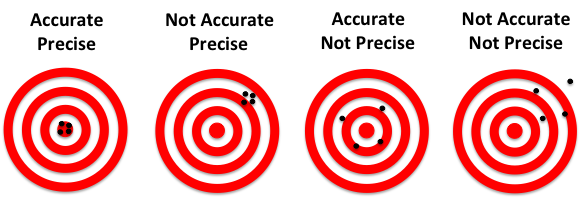
\includegraphics[width=8cm]{acc-prec}
		\caption{accuracy vs precision.}
	\end{figure}
	
	The design of a machine tool or a measurement system has to always consider the \textbf{11 principles for precision} that regards the following key concepts:
	\begin{enumerate}
		\item \textbf{structure}: the structure of the system needs to be stiff with high damping values in order to retain a certain rigidity and thus less degrees of freedom; aspect associated to the structure part are also related to the thermal stability of the system and it's seismic isolation;
		
		\item \textbf{kinematic/semi-kinematic design}: to create a more precisely reliable system  it's necessary to reduce redundant joint between different components (each part has 6 degrees of freedom, but using a joint with more constrains introduce some uncertainty that's the opposite of precision);
		
		\item \textbf{abbé principle}: when aligning measurement system it's important to follow this principle in order not to introduce unexpected side effects;
		
		\item \textbf{direct displacement transducers}: whenever possible it's preferable to measure with a direct transducer, not with a sensor that measure another property that's related to the property itself;
		
		\item \textbf{metrology frames}: this frames that are used to link together the component of the system should be involved in the measurements but should also avoiding the contact with external forces;
		
		\item \textbf{bearings};
		
		\item \textbf{drives/carriages}: in conjunction with the bearings, a system to be put in condition of measure needs to have component with high accuracy that limits the frictions and the thermal effects;
		
		\item \textbf{thermal effects}: whenever possible it's recommended to eliminate/minimise the thermal inputs and drift using stabilization or compensation methods;
		
		\item \textbf{servo drives and control} (CNC): this is a fundamental way to control motion in a repeatable and precise way, especially used in machining systems;
		
		\item \textbf{error budgeting}: in order to improve the way of the system works, it's important to classify different effects in order to understand the relative importance of each effect;
		
		\item \textbf{error compensation}: if it's possible to create a model of the error, it's always good to compensate for it.		
		
	\end{enumerate}
	
	In spite of this 11 principles we realize that, at a fundamental level, there will always be some noise that cannot be eliminated (but can still be reduced). This means that after having designed a system with improved precision it's important to \textbf{identify} and \textbf{quantify} the \textbf{causes leading to non-repeatability}: this is the statistical aspect of precision and represent the so called \textbf{industrial quality}.
	
	\subsection{Autocorrelation}
	
		This day almost all the measures are done using computer and electronic system, so if we consider a displacement sensor it's possible to measure a set of $n$ samples of displacement, each taken after a certain time $\Delta t$. Each sample $x_i$ will necessarily be different from the other, due to it's stochastic nature. At this point to estimate the \textit{real} length of the object to measure we can simply compute the average on the samples token:
		\begin{equation}
			\overline x = \frac 1 n \sum_{i=1} ^n x_i	
		\end{equation}
		This measure will be characterize with a certain variance $\sigma_x^2$; the mean value of the sample will also be a stochastic variable, and so by repeating the experiment itself we can retrieve the variance computed on $m$ measures of $n$ sample each:
		\begin{equation} 
			\sigma^2_{\overline x} = \frac{\sigma_x^2}{m}
		\end{equation}
		
		\begin{SCfigure}[1][bht]
			\centering 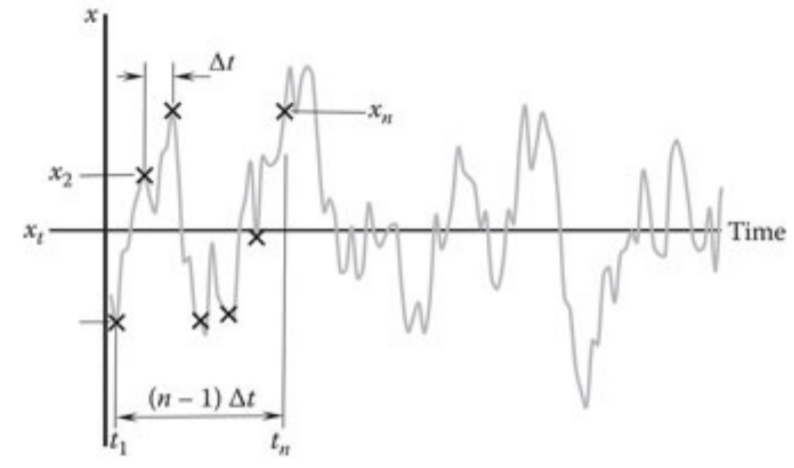
\includegraphics[width=5cm]{autocorrelation}
			\caption{example of values read by a displacement sensor in relation to the time $t$.} \label{fig:design:correlation}
		\end{SCfigure}
	
		As we might see in figure \ref{fig:design:correlation}, reading values in a little time span might result in a correlation between themselves (in fact if we consider a narrow sampling period $\Delta t$, the values registered by the system will be almost be equal), so by increasing the sampling time $\Delta t$ it's possible to get measures that are less correlated between each others. In particular, to solve this problem, it's possible to create the \de{autocorrelation function} $R_{xx}$ whose purpose is to define the minimum sampling time $\Delta t$ that generates uncorrelated data. This particular function is defined by computing the average of a signal with itself translated in time by a constant value $\tau$, so by doing
		\begin{equation}
			R_{xx}(\tau) = \frac 1{T-\tau} \int_0^{T-\tau} x(t) x(t-\tau) \, dt
		\end{equation}
		This particular function is interesting, because we can see that for $\tau = 0$ it simply compute the variance $\sigma_x^2$, however it happens that by incrementing the parameter $\tau > 0$ the function decrease following an exponential decay with time a time constant equal to $\tau_0$ and so the asymptotic value is zero; note that this behaviour is not a true value, but just an asymptotic limit, as it can be seen in figure \ref{fig:design:correlation-b}.
	
		\begin{SCfigure}[1][bht]
			\centering 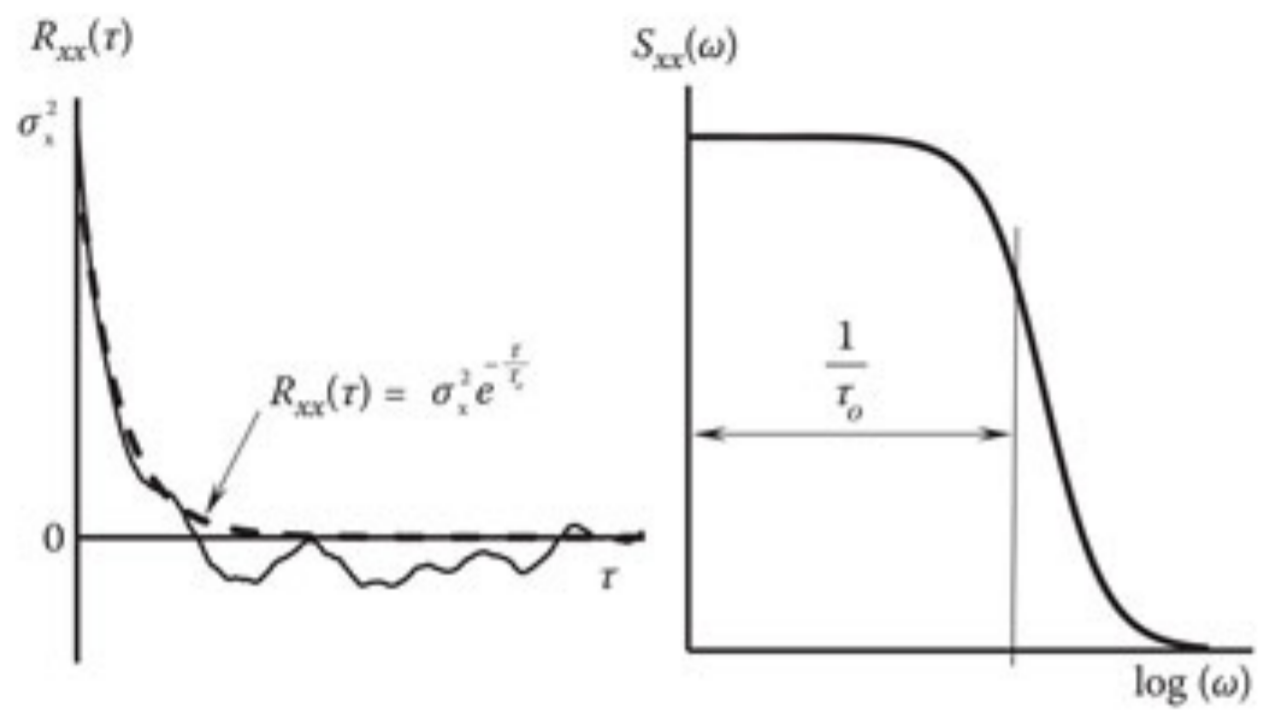
\includegraphics[width=5cm]{autocorrelation-b}
			\caption{trend of the function $R_{xx}$ and $S_{xx}$ read by an instrument.} \label{fig:design:correlation-b}
		\end{SCfigure}
		
		By considering the asymptotic value of the autocorrelation function, so by describing it as $R_{xx}(\tau) = \sigma_x^2 e^{-\frac{|\tau|}{\tau_0}}$ it's possible to compute the power spectral density $S_{xx}$ in the domain of the frequency that's equal to
		\begin{equation}
		\begin{split}
			S_{xx}(\omega) & = \frac{\sigma_x^2}{\pi} \int_0^\infty e^{-\frac{\tau}{\tau_0}} \cos(\omega \tau)\, d\tau = \frac{\sigma_x^2}{\pi \tau_0} \frac 1 {1 + (\omega \tau_0)^2} \\ & = \frac{S_0}{1 + (\omega \tau_0)^2}
		\end{split}
		\end{equation}
		This function is useful to determine that the value $\tau_0$ represents the \textbf{minimum sampling time} for consecutive samples to get the uncorrelated. Going back to the original statement of this section in order to get uncorrelated values we need to use a sampling time $\Delta t > \tau_0$.
		
		By this it consequent that, chosen a time $T$ on which the measure system saves data, the maximum number of uncorrelated sample that can be used for computing some specification on the system is equal to $n = T/\tau_0$, and so with them we can estimate the standard deviation $\sigma^2_{\overline x}$ on the averaged signal:
		\[ \sigma_{\overline x}^2 = \frac{\sigma_x^2}{T/\tau_0} \qquad \Rightarrow \quad \sigma_{\overline x} =\sigma_x \frac{\sqrt{\tau_0}}{\sqrt {T}} = \frac{P_0}{\sqrt {T}} = P_0 \sqrt{(BW)_m} \]
		As stated in this expression, by computing the square root on the variance it's possible to get the standard deviation of the system, and it's possible to see that's related to the \textbf{intrinsic signal noise} $P_0$ (property of the system) and to the square root of the acquisition time $T$ (if on denominator) or on the \textbf{measure bandwidth} $(BW)_m = 1/T$ (if on numerator). \\
		Note that the standard deviation is related to the square root of the acquisition time, so to increase the deviation $\sigma_{\overline x}$ (and so the precision) by a factor of 10, it will require 100 times more time, with a significantly increase of costs.
		
	\subsection{Limits of precision}
		
		As yet described, a limit of precision is the cost because it limit the acquisition time $T$ that could have reduced the standard variation $\sigma_{\overline x}$, but this is not the lonely effect.
		
		Virtually all precision measurements pass through electronics that are subjected to the so called \textbf{Johnson's noise} that's related to the random movement of the atoms that compose the structure, and so in general it depends on the temperature $T$ of the system. Consider for example a resistor $R$, it's thermal noise $P_{0,V}$ depends also on the Boltzamnn's constant $k = 1.38\cdot 10^{-3} J \cdot K^{-1}$ and the sampling bandwidth $(BW)_s$ as described by the equation
		\begin{equation}
			P_{0,V} = 2 \sqrt{RkT (BW)_s}
		\end{equation}
		
		When combining many electric and passive components, their noise sum up to combine into a \textbf{pink noise} (like a white noise, but with more components on higher frequencies) whose spectral density is defined by the function
		\[ G(f) = \frac C f + G_0 \]
		Integrating this function over the frequency band of interest gives the variance $\sigma^2_V$ associated to this particular kind of noise
		\begin{equation}
			\sigma_V^2 = \int_{f_1}^ {f_2} G(f)\, df = C \ln \left( \frac{f_1}{f_2} \right) + G_0 \big(f_2-f_1\big)
		\end{equation}
		The truth that this equation wants to tell us it that is difficult to maintain precision over a long time, because the difference of frequencies $f_2-f_1$ (multiplied by $G_0$) will increase the variance.
		
		Another phenomenon that limit the precision of an instrument is the granular nature of current (that's made of flowing electrons); this effect is dominant for high currents $I$ and bandwidth $(BW)_s$ and determine a so called \textbf{shot noise} $P_{0,I}$ that's equal to		
		\[ P_{0,I} = \sqrt{2qI (BW)_s}\]
		where $q = 1.602\cdot 10^{-19} C$ is the charge of an electron.		
		\vspace{3mm}
		
		Pink noise and shot noise are the limiting factors on precision measurements where a phenomenon is converted through a transducer into a voltage or current. Much better precision can be exploited by converting a phenomenon into a value through time (needed, as example, for charging a capacitor or for a beam of light to travel a distance...) and not voltage/current; this time precision can reach value of $10^{-11} s$, increasing the precision of the overall system.
	
	
	
	
	
	
	
	
	
	
	
	
	
	
	
	
	
	

%	\chapter{Precision Systems}
	This chapter is focused on system-related aspects that are relevant to \de{precision systems}, in particular related to the abbe, sine and cosine errors, the kinematic design and the flexure hinges.
	
\section{Alignment: Abbe, sine and cosine errors}
	
	Alignment errors are arising every time we need to align a measurement system and the subject of study: we have to be aware of this kind of error in order to detect them and control/reduce them. In particular the \de{Abbe} error arise every time there's an offset between the object to be measured and the system that perform the measure.
	
	Doing a low-volume production (or with high added value products) it's possible to rely on a manual inspection held by highly trained technician in order to ensure a certain level of quality; considering instead a mass production a handmade check of each component it's not possible due to a fully automated manufacturing and assembly for which there is a little space for adjustment: repeatability and precision must be designed into the product in order to have a high quality.
	
	\paragraph{Abbe's error} Common alignment errors are related to the \textbf{Abbe's error} associated  to it's principle stating that \textit{"the measurement line shall be collinear with the line of motion"}.
	
	\begin{SCfigure}[1][bht]
		\centering
		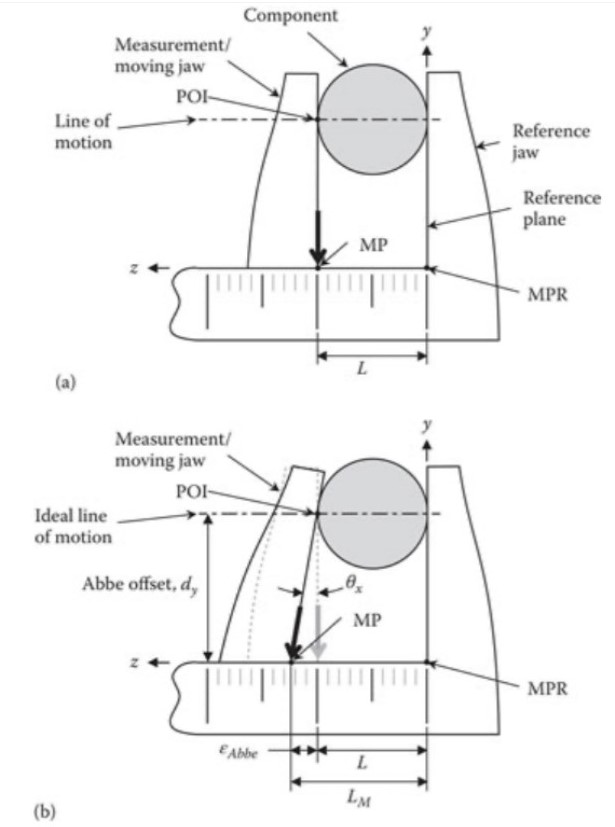
\includegraphics[width=6cm]{abbe-scheme}
		\caption{scheme used to understand the Abbe's error on a calliper. $(a)$ is a correct calliper while $(b)$ is affected by the error.} \label{fig:ps:abbescheme}
	\end{SCfigure}
	An example of this error can be seen in the calliper as in figure \ref{fig:ps:abbescheme}, where the goal is to measure the \textbf{Point of Interest} POI by reading the \textbf{Measurement Point} MP in respect to the Measurement Point \textbf{Reference} MPR. \\
	At a nominal level the two jaws of the calliper should be parallel, and so the point of interest is measured by only looking at the measurement point, but in reality misalignment are always present: this introduce an error $\abbe$ of the measurement point respect to the point of interest. Related to this error we can compute a linear relation but also an expression considering a second order term (that for low error alignment value $\theta_x$ can be neglected), obtaining
	\begin{equation}
		\abbe = d_y \tan\theta_x - \underbrace{L \left(\frac 1 {\cos\theta_x} - 1\right)}_\textrm{2nd ord. term}
	\end{equation}
	
	In reality things are even more complicated: Abbe's error are related to two angle in the 3D space, the so called \textbf{pith} and \textbf{yaw}
	\begin{equation}
	\begin{split}		
		\abbe & = d_y \tan\theta_x - L \left(\frac 1 {\cos\theta_x} - 1\right) + d_x \tan\theta_y - L \left(\frac 1 {\cos\theta_y} - 1\right) \\
		& = d_y \tan\theta_x + d_x\tan\theta_y - L\left( \frac 1 {\cos\theta_x} + \frac 1 {\cos\theta_y} - 2 \right)
	\end{split}
	\end{equation}
	
	\begin{SCfigure}[2][bht]
		\centering
		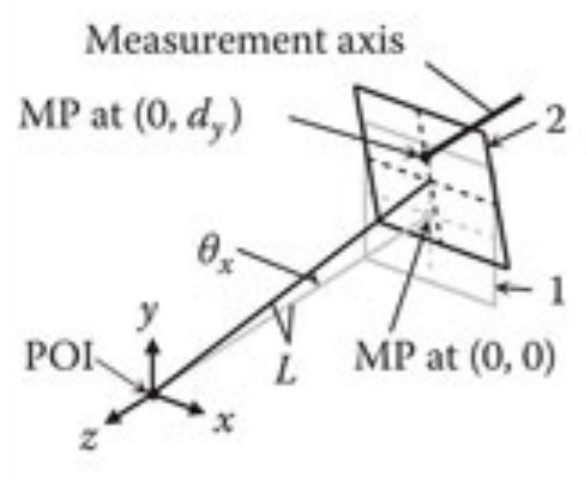
\includegraphics[width=3.5cm]{abbe-error}
		\caption{scheme used to understand the equation of the Abbe's error.} 
	\end{SCfigure}

	In order to eliminate the Abbe's error we can compensate by adding two more sensor (to determine $\theta_x,\theta_y$) that can determine the error $\abbe$. The same goal can be performed by analysing a sample problem: known it's value $L_m$, the computed measures is
	\[ L = L_m - d_y\tan\theta_x - d_x\tan\theta_y \]
	By evaluating this expression in two points (considering that an error, like $d_x\tan\theta_y$, can be consider negligible in respect to the other) by measuring an object more internal and external, we have a mathematical system that can be used in order to determine the unknown value $\theta_x$ and $L$. This method, in order to be successful, must consider that the angles $\theta_x$ and the length $L$ of the measure are invariant while changing the position of the sample.
	
	A smarter way to avoid the Abbe's error is just by doing a design choice minimizing the offset, so by making the line of motion collinear with the line of measurement.
	
	\paragraph{Cosine and sine error} The \de{cosine} error happens every time the measurement line is not parallel to the line of action. Considering the example of the measure of a length with a rule (as in figure \ref{fig:ps:cosineerror}) we can see that the measured length $L_m$ is different from the \textit{real} length $L$ of the object that we want to study, and in particular we can then evaluate the difference in order to define the cosine error $\varepsilon_{\cos}$:
	\begin{equation}
		L = L_m \cos\alpha \qquad \Rightarrow \quad \varepsilon_{\cos} = L_m - L = L_m \big(1-\cos\alpha\big)
	\end{equation}
	
	\begin{SCfigure}[1.3][bht]
		\centering
		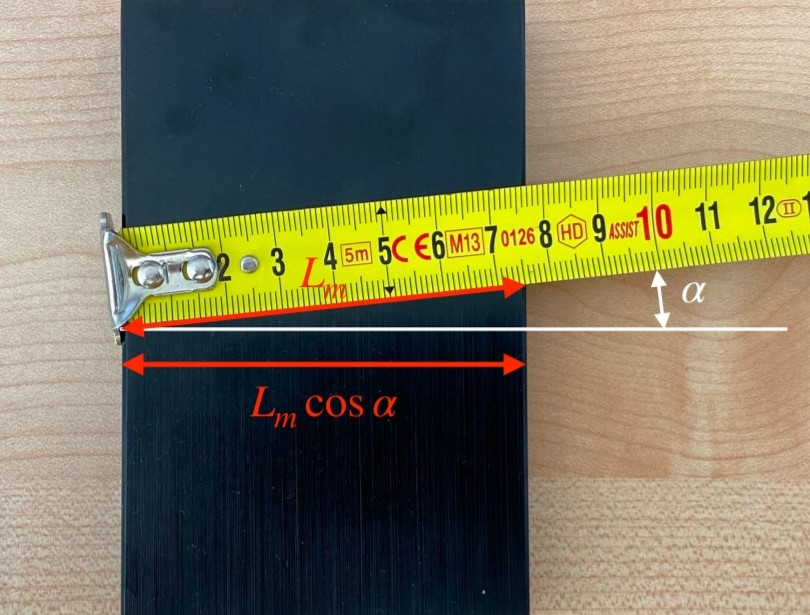
\includegraphics[width=5cm]{cosine-error}
		\caption{cosine error on a length measure.}  \label{fig:ps:cosineerror}
	\end{SCfigure}
	Extending the cosine error to a spatial environment we can compute  the error considering two angle $\alpha_x$ and $\alpha_y$ that can lead to an error:
	\begin{equation}
		\varepsilon_{\cos} = L_m\big(1-\cos\alpha_x\cos\alpha_y\big)
	\end{equation}
	\vspace{3mm}
	
	The \de{sine} error typically occurs when a physical contact is necessary for the measurement, like while dealing with the jaws of the calliper. By referring to figure \ref{fig:ps:sineerror} we can see that the error $\varepsilon_{\sin}$ is different in base of the geometry of the contact; considering as an example a flat-on-flat contact we can evaluate the error as
	\begin{equation}
		\varepsilon_{\sin} = \frac {w_z}2\sin\alpha_x + \frac{w_x}{2}\sin \alpha_z
	\end{equation}
	while considering instead a point contact the error reduces to the expression
	\begin{equation}
		\varepsilon_{\sin} = \frac {w_z}2\big(1-\cos\alpha_x\big) + \frac{w_x}{2}\big(1-\cos\alpha_z\big) = \frac{w_z}{2}\big(2-\cos\alpha_x-\cos\alpha_z\big)
	\end{equation}	
	
	
	\begin{SCfigure}[1.3][bht]
		\centering
		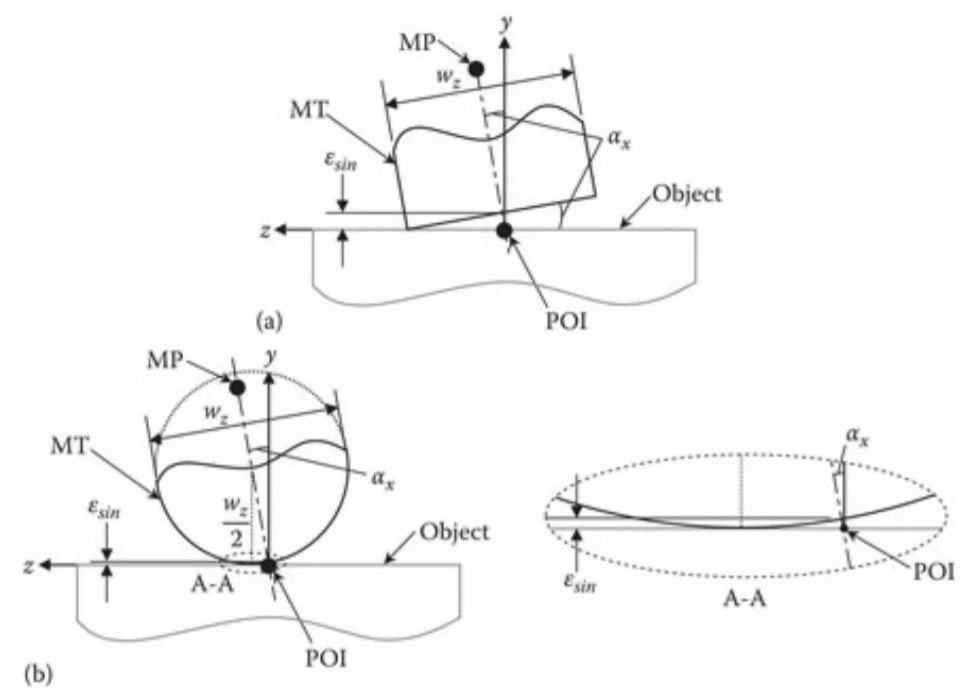
\includegraphics[width=5cm]{sine-error}
		\caption{sine error on a surface measure considering a flat-on-flat contact $(a)$ or a point contact $(b)$.}  \label{fig:ps:sineerror}
	\end{SCfigure}

	\paragraph{Alignment errors} In general Abbe's, cosine and sine errors are not mutually exclusive, so they can occur at the same time (Abbe's related to the offset, cosine due to a scale line not parallel to the  line of motion and the sine related to the angle between the moving jaw and the object).
	
	While designing measurement system it's important to determine all the specification that are useful to calculate the error factors that should be less then a decided value; this gives a suggestion on how to chose tolerances of the products.
	
	\begin{figure}[bht]
		\centering
		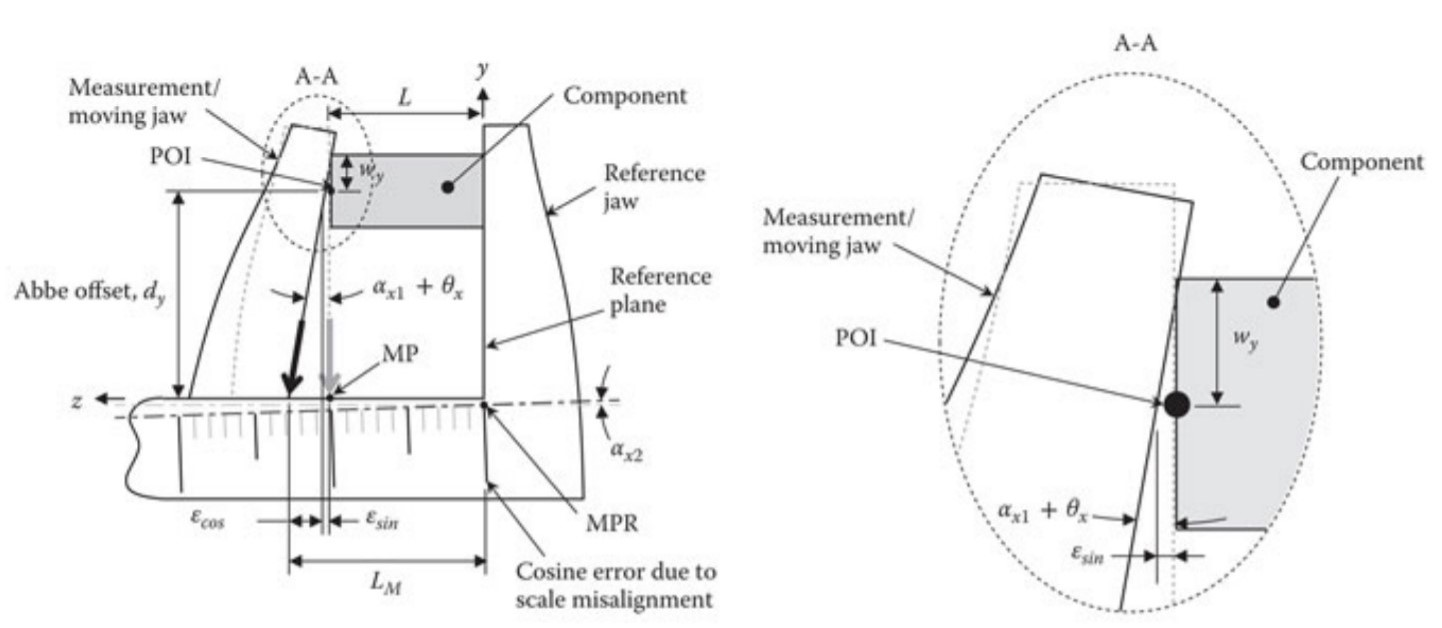
\includegraphics[width=10cm]{comb-errors}
		\caption{example of the combination of Abbe's, cosine and sine errors in a calliper.}
	\end{figure}
	
\section{Kinematics}
	
	In order to have a repeatable positioning it's important to minimize the internal stress by pursuing an isostatic design. When designing a system the kinematic analysis provides an understanding between the functional relationship between parts of mechanism, on how these parts are interconnected and how they move relative to each other.
	
	For example an unilateral constraint is represented by an inequality such $f(x,y,z) \geq 0$: in this step we usually consider bodies as \textbf{rigid}, so by considering part that are stiff enough in order to consider their deformation negligible in respect to the typical range of motion of the system. In precise machine it's important to consider all contact as rigid. \\
	In kinematic design we can assume that each	point of contact between two rigid bodies corresponds to a mutual constraint. In general if $f_j$ is the number of degrees of freedom of a joint $j$ having $n_{p_j}$ lowest number of contact point, than it's true that
	\begin{equation}
	\begin{split}
		\textrm{planar kinematics:}& \qquad f_j = 3 - n_{p_j} \\
		\textrm{spatial kinematics:}& \qquad f_j = 6 - n_{p_j} \\
	\end{split}
	\end{equation}
	
	Considering the more complex scenario of two line (straight or arcuate) contact, this is kinematically equivalent to two point constraints applied to any two different points along the contact line. 
	
	\begin{SCfigure}[2][bht]
		\centering
		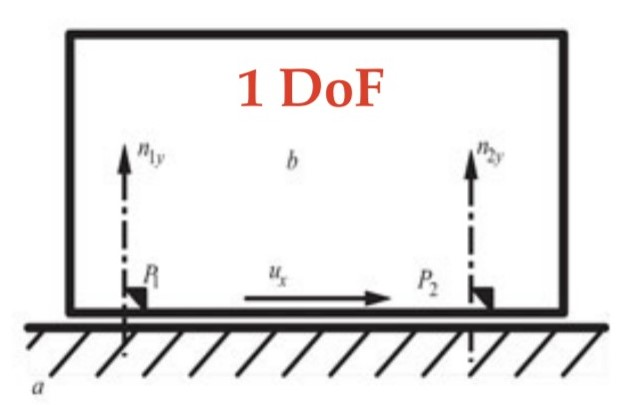
\includegraphics[width=3.5cm]{planar-contact}
		\caption{the contact of a body with straight line on a straight surface leads to two point constrains in order to have 1 degrees of freedom.}
	\end{SCfigure}
	
	\paragraph{Mobility of mechanisms} Considering now  a combination of $n$ rigid bodies constrained by $j$ joints can lead to a movable or immovable system. The net mobility of the mechanism is its number of degrees of freedom and can be calculated according to Tchebytchev as
	\begin{equation}
		M = D\big(n-1-j\big) +\sum_i f_i = D\big(n-1\big) -\sum_j n_{p_j}
	\end{equation}
	where $D= 6$ for spatial mechanisms while $D= 3$ for planar kinematics. If $M>0$ then the mechanism is movable, for $M = 0$ the system is immovable while $M < 0$ it's over-constrained and so, in a real application, the structure will be subjected to unknown internal stresses that cannot be quantified (and so leading to imprecision).
	
	The Tchebytchev should be used with caution when dealing with bodies that present singularities	
	
	
	
	
	
	
	
	
	
	
	
	
	
	
	
	
	
	
	
	
	
	
	
	
	
	
	
	
	
	

\section{Flexure hinges}
	
	
	
	
	
	
	
	
	
	
	
	
	
	
	
	
	
	
	
	
	
	
	
	
	
	
	
	
	
	
	
	
	
	
	
	
	
	
	
	
	
	
	
	
%	\chapter{Measurements}
\section{Dimensional metrology}
	The \de{dimensional metrology} is the study of geometrical measurements (such lengths, areas, roughness). The \textbf{confidence} in the dimensions of this measurement systems is critical for their operation and establishes an agreement between the vendor and the customer on the quality being traded.
	
\subsection*{Length standards}
	A \textbf{measurement standard} is a practical realization of the definition of a measurement unit. As example the first international standard of length was a platinum-iridium bar names \textit{International Prototype Metre}; now the definition is changed and a meter is the length of the path travelled by the light in a vacuum in $1/299\,792\,458s $ (and so it's now a derived unit).
	
	The idea of standard allows the definition of the traceability chains (usually consisting of 4 levels) that's transferred between levels using calibration.
	
	\begin{SCfigure}[1][bht]
		\centering 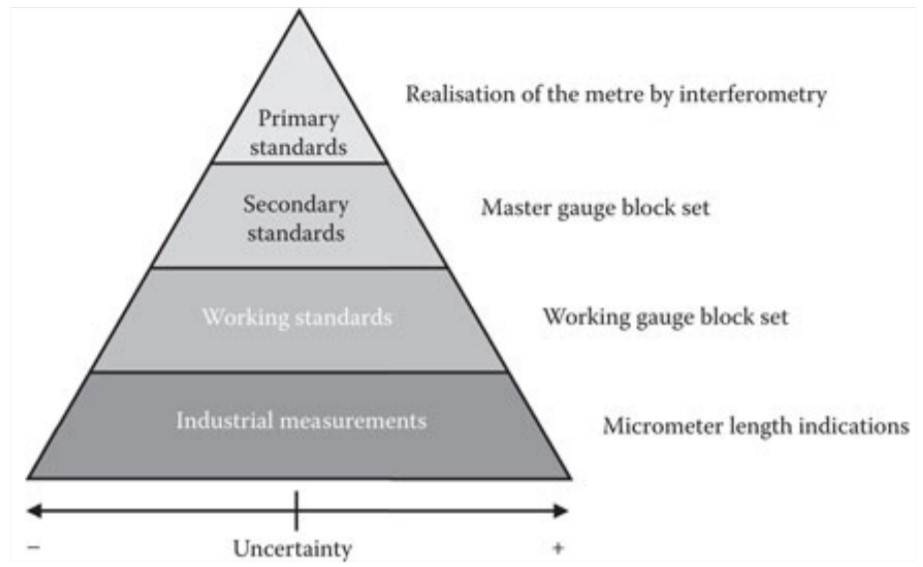
\includegraphics[width=7cm]{trace-levels}
		\caption{pyramid representing the 4 levels of traceability chain.}
	\end{SCfigure}
	
	A length standard can consist of a edge gauges block of, more easily, using \textbf{line standard} which provide the reference lengths as the distance between two parallel lines on the surface of the object (so, as example, a simple ruler or calliper). The line standard is often used for calibrating the scales of optical vision system.
	
	\begin{SCfigure}[2][bht]
		\centering 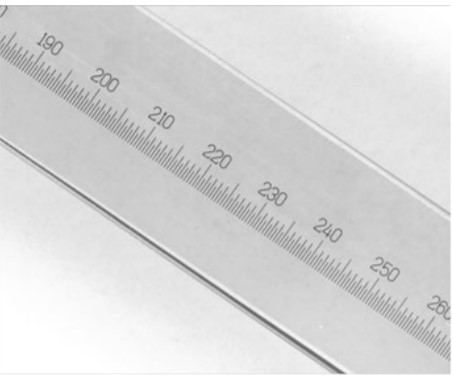
\includegraphics[width=4cm]{ruler}
		\caption{example of a line length standard.}
	\end{SCfigure}
	
\subsection{Displacement sensors} 
	The contact displacement sensor measure the linear position of an object by physically contacting its surface with a prove. An example of digital comparator of displacement is the \textbf{LVDT} (\textit{Linear Variable Differential Transformer}) transducer. In this case the displacement is related to the motion of a movable electromagnetic core that determines a change of mutual inductance between the primary and secondary coils that's then measured by a voltmeter.
	
	\begin{SCfigure}[2][bht]
		\centering 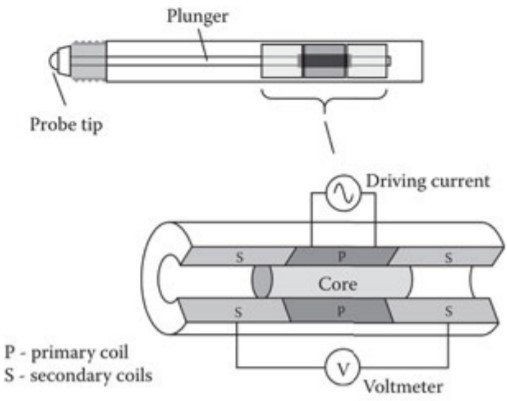
\includegraphics[width=4cm]{lvdt}
		\caption{functional schematic of an LVDT displacement sensor.}
	\end{SCfigure}
	
	Displacement can also be measured using \textbf{encoders} that determines a (relative or absolute) position in digital format by counting the number of optical/magnetic/inductive pulses. \\
	Relative encoder are easier to implement and requires only two tracks to measure the displacement and it's direction, but every time it's necessary to restart from a known position. Considering instead an absolute encoder the minimum number of tracks to measure a length $l$ with a resolution $r$ is $\lceil \log_2 (l/2) \rceil $ (for example to measure a length of $l=1m$ with a resolution of $r=1\mu m$ the minimum number of tracks is 20); this measure relates also to the number of bits representing the measure.
	
	In general absolute encoders don't presents masks with a binary encoding, but they use the \textit{Gray code} (in order to avoid the problem of multiple wrong reads of the sensor while being near to the commutation stage) that assures only one change of bit for each step.
	
	\begin{SCfigure}[1][bht]
		\centering 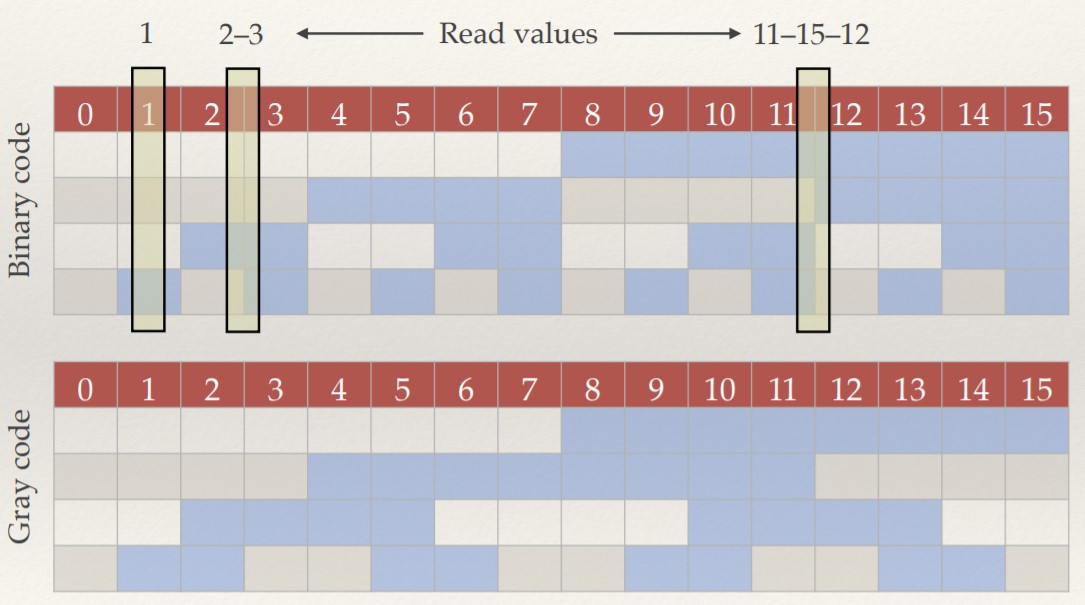
\includegraphics[width=8cm]{greycode}
		\caption{binary code vs Gray code masks for absolute encoders.}
	\end{SCfigure}
	
	\paragraph{Non-contact displacement sensors} The previous explained measurement method for displacement require a contact between the system and the object to be probed, but it possible to create systems contact free using the following measurement principles:
	\begin{itemize}
		\item \textbf{light interferometry}: in this case the system  consists of a laser source that splitted by a beam into two retroreflectors (as shown in figure \ref{fig:meas:interferometer}).		
		
		\begin{SCfigure}[1][bht]
			\centering 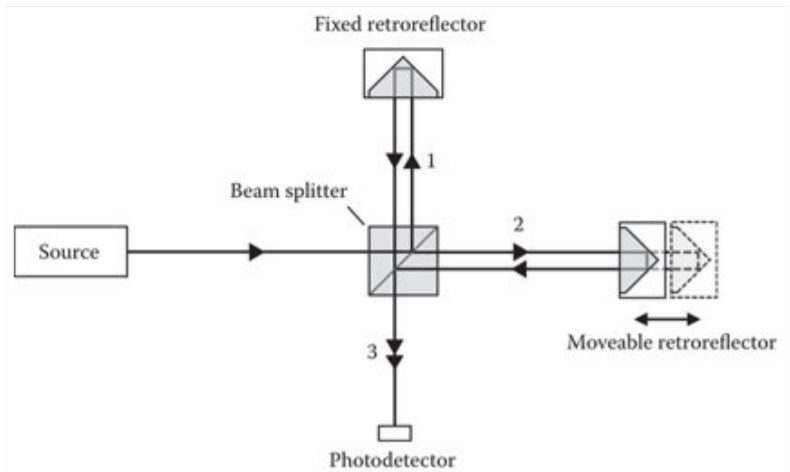
\includegraphics[width=6cm]{las-sys}
			\caption{schematic representation of a laser interferometer.} \label{fig:meas:interferometer}
		\end{SCfigure}
		 
		 The intensity of the interference signal is function of the phase difference between the superimposed beams ($0^\circ$ for constructive interference, $180^\circ$ for the destructive one). The intensity of the interference signal repeats with displacements of the retroreflector equal to one half of the wavelength $\lambda$ of the light beam and, by interpolation of the phase within a fringe period, it's possible to achieve sub-nanometre resolutions. In general the resolution is great ($10nm$) with a range up to hundreds of meters (and so it has a huge dynamic range);
		 
		 \item \textbf{light intensity}: this system has an high resolution but a limited range  and uses fiber optics carrier to enlight the surface and measure the reflected light;
		 \begin{figure}[bht]
		 	\centering 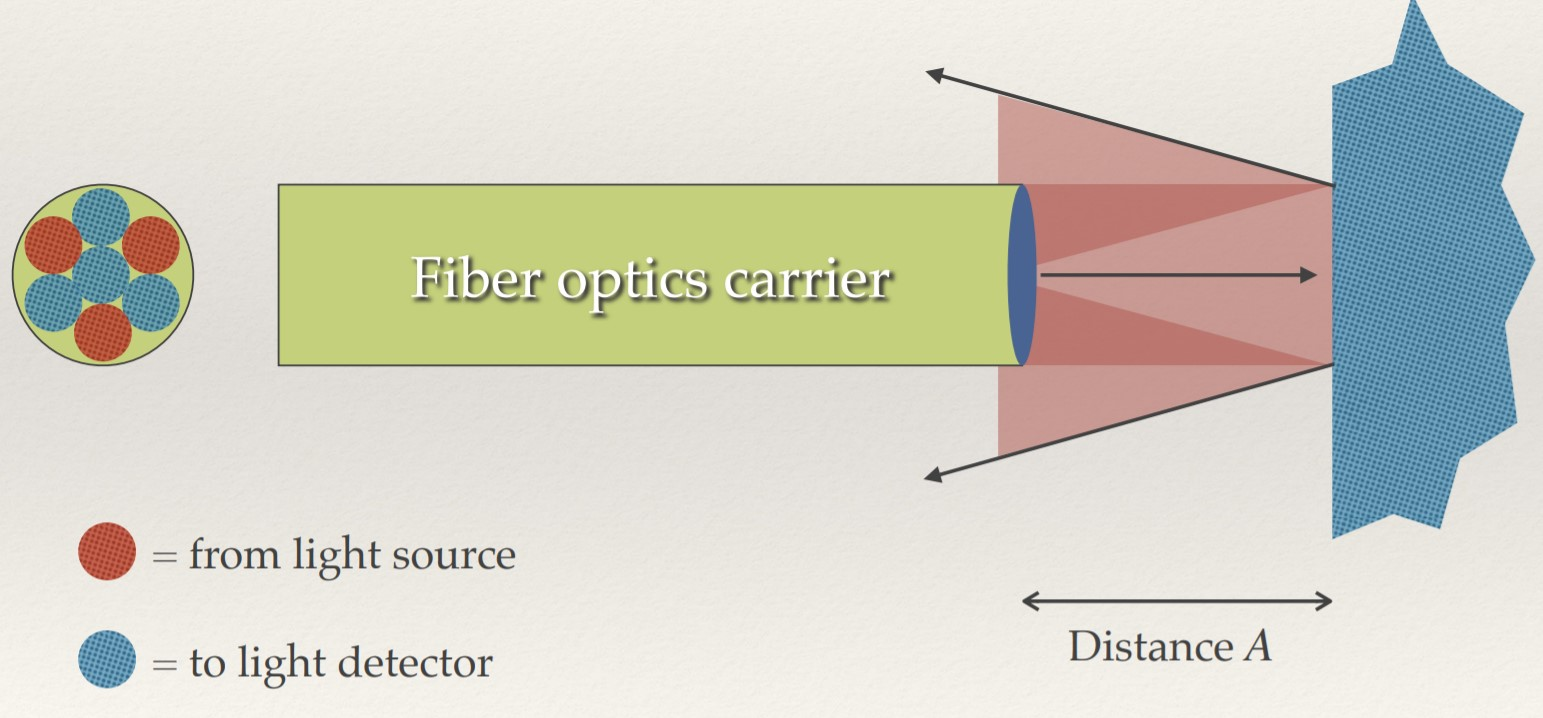
\includegraphics[width=7cm]{fibermeasure}
		 	\caption{schematic representation of a light intensity measurement system.}
		 \end{figure}
	 
	 	\item \textbf{trilateration}: in this case we use a line pixel array to detect the shift of the reflected light source.
	 	
	 	\begin{SCfigure}[1][bht]
	 		\centering 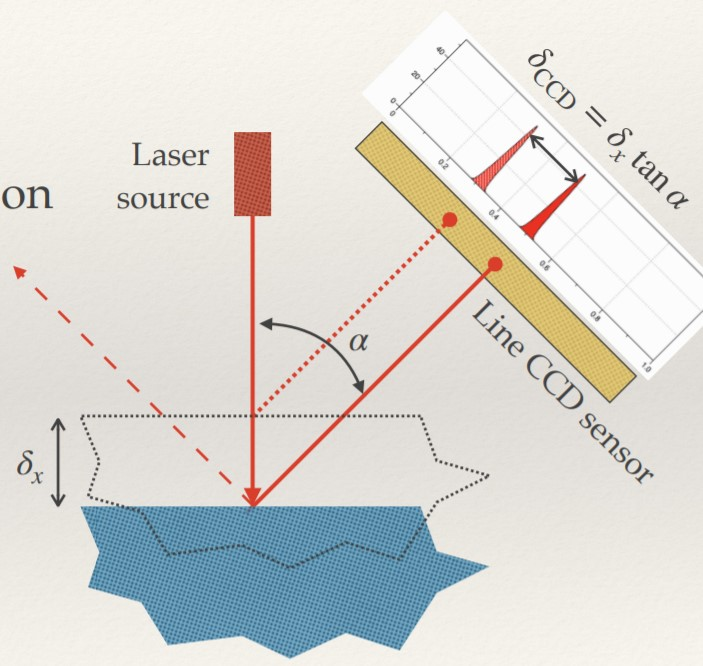
\includegraphics[width=5cm]{trilateral}
	 		\caption{schematic representation of a trilateration measurement system.}
	 	\end{SCfigure}		
	\end{itemize}
	
\subsection{Form measurement}
	\paragraph{Straightness and roundness} The \de{straightness} is measured as lateral deviation along a displacement; in this case the reference line can be computed by interpolation (by computing as example the least-square line). With an analyses of the surface we can define the parameters such the peak-ref deviation $STR_p$, the valley-ref deviation $STR_v$, the peak-valley deviation $STR_t = STR_p + STR_v$ and the RMS deviation $STR_q$.
	
	\begin{SCfigure}[2][bht]
		\centering 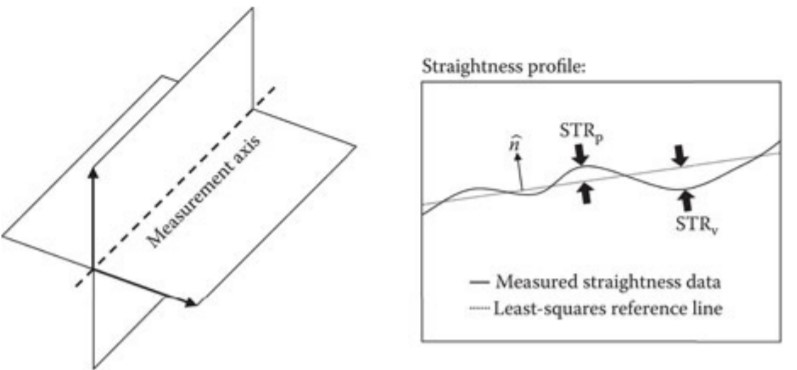
\includegraphics[width=6cm]{straightness}
		\caption{measurement axis and straightness profile with main parameter of this kind of form measure.}
	\end{SCfigure}
	
	Similarly we can define the same parameters for a circular surface determining so the \de{roundness} $RON$ of the piece.
	
	\textbf{Flatness} can be regarded as the straightness in two dimension (on a surface, not a axis), while \textbf{parallelism} defines a tolerance zone respect to a datum, rather than respect to the reference line.
	
	\begin{SCfigure}[2][bht]
		\centering 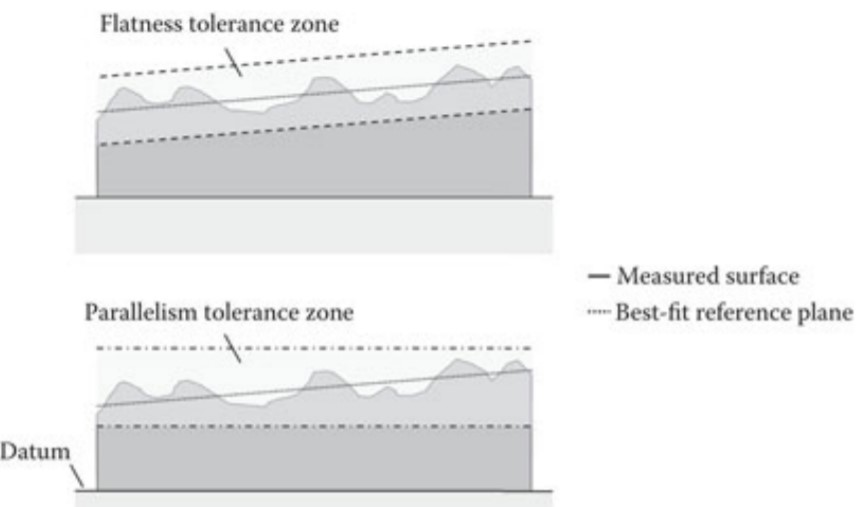
\includegraphics[width=8cm]{flat-par}
		\caption{flatness and parallel zone tolerance for a piece.}
	\end{SCfigure}
	
	In order to asses the flatness we can use an optical flat that use the patterns of the fringes due to light interferometry to determine the flatness of the surface.
	
	\begin{SCfigure}[2][bht]
		\centering 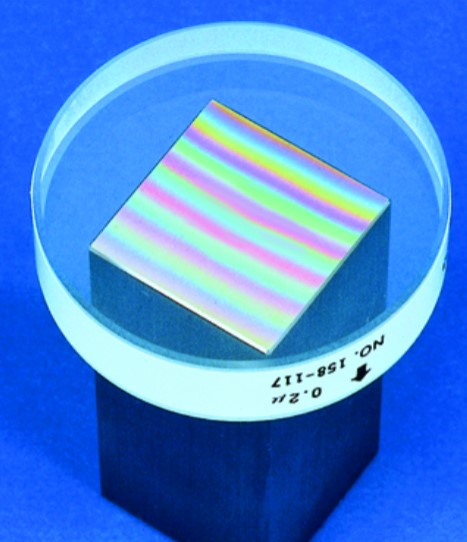
\includegraphics[width=3cm]{opt-flat}
		\caption{example of an optical flat system to measure flatness.}
	\end{SCfigure}
	
	\paragraph{Roughness} To determine the \de{surface roughness} of a surface we need to split it's topography (all wavelength) into surface texture (short wavelength) and  surface form (long wavelength associated to the baseline). In particular the roughness is a one dimensional texture measured along a single scan line.
	
	\begin{SCfigure}[2][bht]
		\centering 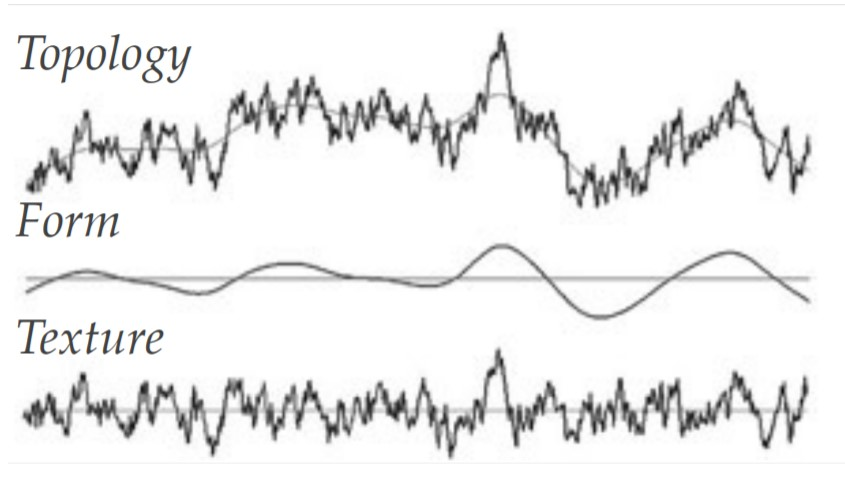
\includegraphics[width=5cm]{rough-top}
		\caption{topology, form and texture surface for a piecea.}
	\end{SCfigure}

	Texture measure can be either be contact (stylus sliding orthogonally to the surface) or contact-less (optical analysis that's intrinsically bi-dimensional). In general non contact texture instruments provides a height map image of the surface that can be easily analysed and can convey a lot of information. In general non contact texture instruments have a limitation in the resolution $r$ (compared to the contact one) that depends on the numerical aperture $A_n = n \sin\alpha$ following the relation $r = k \lambda /A_n$ (where $k=0.61$ is the Raylight criterion,$\lambda$ is the light wavelength and $n$ is the refractive index of the optic).
	
	In general to compute the parameter $Ra$ associated to the \textbf{surface roughness} we consider the equation
	\begin{equation}
		Ra = \frac 1 L \int_0^L |z(x)| \, dx
	\end{equation}
	where $L$ is the reference length on which we compute the parameter and $z(x)$ represent the deviation of the surface from the centre line.
	
	\paragraph{Reversal principle} A simple way to separate error is to use the \de{reversal principle} that consist on a double measure reversing the measurement system.
	
	\begin{SCfigure}[2][bht]
		\centering 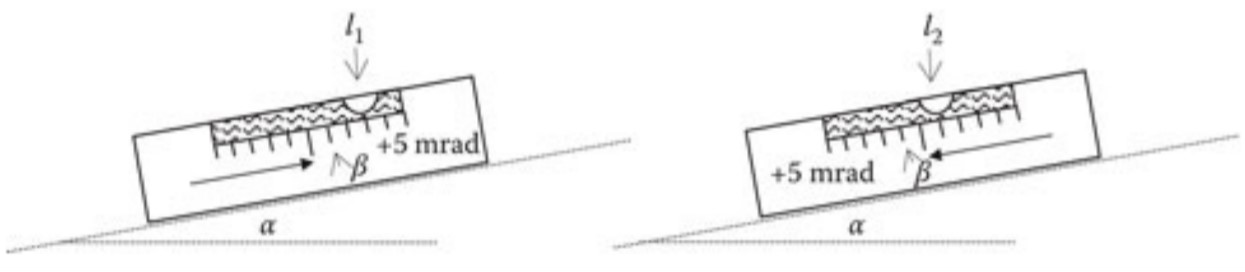
\includegraphics[width=7cm]{rev-princ}
		\caption{application on where the reversal principle can be useful.}
		\label{fig:meas:reversal}
	\end{SCfigure}
	
	Let's consider the practical case shown in figure \ref{fig:meas:reversal} of the instrument shown that allows to compute the angle $\alpha$ of the inclined plane on which is placed by transducing the rotation in the displacement $l$. If the measurement system present an imperfection that translates to an addition of the angle $\beta$ to the measure, this offset error can be compensated using the reversal principle.\\
	Knowing that the first measure gives a displacement $l_1 = \alpha + \beta$, by reversing the orientation of the instrument the output becomes $l_2 = \alpha - \beta$: this allows to calculate more precisely the value $\alpha$ and the error $\beta$ introduced by the system as
	\[ \alpha = \frac{l_1 + l_2}{2} \qquad \ \qquad \beta = \frac{l_1-l_2}{2} \]
	Once that the error $\beta$ is computed and known there's no need to perform this operation every time we want to do a measure.
	
	
	
	
%	\chapter{Disturbances}
\section{Force loops}
	
	Whenever designing a precise system, an important key aspect to keep in mind is to decouple as much as possible measurements and side effects and in particular the forces.
	
	In fact there are no infinitely rigid material and so any force results in a displacement which can affect the measurement or precision when its magnitude is comparable with the resolution. Also we have to keep in mind that every mechanical system obey the Newton's first law and so we can recognize a balanced \textbf{loop of forces} acting within, and in particular we need to realize
	\begin{itemize}
		\item which forcer are related to the process performed by the system;
		\item what are the paths followed by those forces.
	\end{itemize}
	All force loops, due to the Newton's law, must be closed. Visualizing force loops helps in designing the structure and the interfaces, so that the process forcers  result in minimal deformations along all the force loop. In particular we have to consider that bearing (or in general element with lower elastic stiffness) subject to the force (due to the loop) doesn't deform with values out of the resolution range. In  general any deformation (in particular the one associated to thermal expansion due to temperature gradients that cannot be measured) along the loop directly produces a measurement error.
	
	\paragraph{Functional independence design principle} A good design tries to split functions into different subsystems and, to make their performances independent, so that one subsystem can be tuned/calibrated/adjusted independently without affecting the others.
	
	\paragraph{Metrology loop} A \de{metrology loop} is a structural loop of all elements whose dimensional changes would not be measure and the better is to have them as short as possible. With this said then it means that any mechanical play shall be kept out of it and be reduced.
	
	Often forces and metrology loops have different/incompatible requirements; as example a linear encoder (metrology loop) must be insensitive temperature (and so we can use INVER alloy) while the structure must be resistant and with high damping (and so cast iron is \textit{better}). This is another reason to apply the functional independence design principle and keep at minimum the interfaces between metrology and force (structural) loops; minimum interfaces often means (quasi-)kinematic mounts.
	
	\paragraph{Thermal loop} Path across an assembly of mechanical components which determines the relative position between specified objects under changing temperatures. Considering $L_s$ the length of components whose expansion relates to an expansion and and $L_c$ the one that close the loop, it means that
	\[ \Delta L = \sum_i L_{s,i} \alpha_i \, \Delta T_i - \sum _j L_{c,j} \alpha_j\, \Delta T_j \]
	This error can be compensated if we compute the temperatures of each part of the system (and in order to improve this we have to increase thermal conductivity to reduce thermal gradients). Another technique that can be used is to design symmetric structures that better rejects effects of thermal gradients with the drawback of having a larger, heavier, slower and more costly system.\\
	Using kinematic mounts two components can be made thermally invariant at one point known as \textbf{thermal center} (figure \ref{fig:dist:thermalcenter}).
	
	\begin{SCfigure}[2][bht]
		\centering 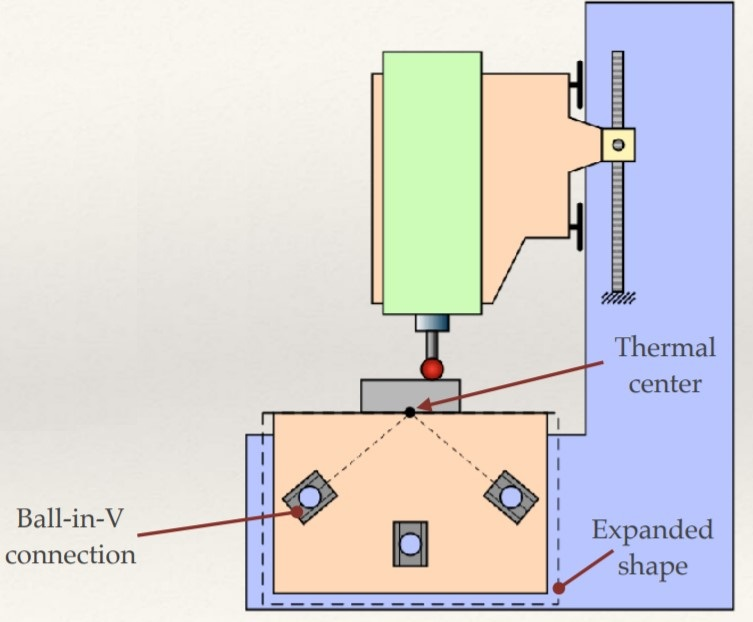
\includegraphics[width=6cm]{thermal-center}
		\caption{example of kinematic mount that allow to compensate temperature variation.} \label{fig:dist:thermalcenter}	
	\end{SCfigure}
	
	\paragraph{Maximum permissible error} Displacement and length precision measurement system declare their accuracy in form of \de{maximum permissible error}, a contractual figure to be verified upon first installation; there is no predefined methodology fo assessing this parameter and it's definition/calculation depends on the vendor and the manufacturer. In general it's not a good to choose a system over another based on the maximum permissible error declared  by the vendor.
	
	
\section{Materials selection}
	
	\de{Ashby maps} are 2D plot reporting pairs of related properties (like strength vs density) in $\log-\log$ plots reporting classes of materials as clouds (figure \ref{fig:dist:ashby}), making easier to understand which materials might suit for a certain application.
	
	\begin{figure}[bht]
		\centering 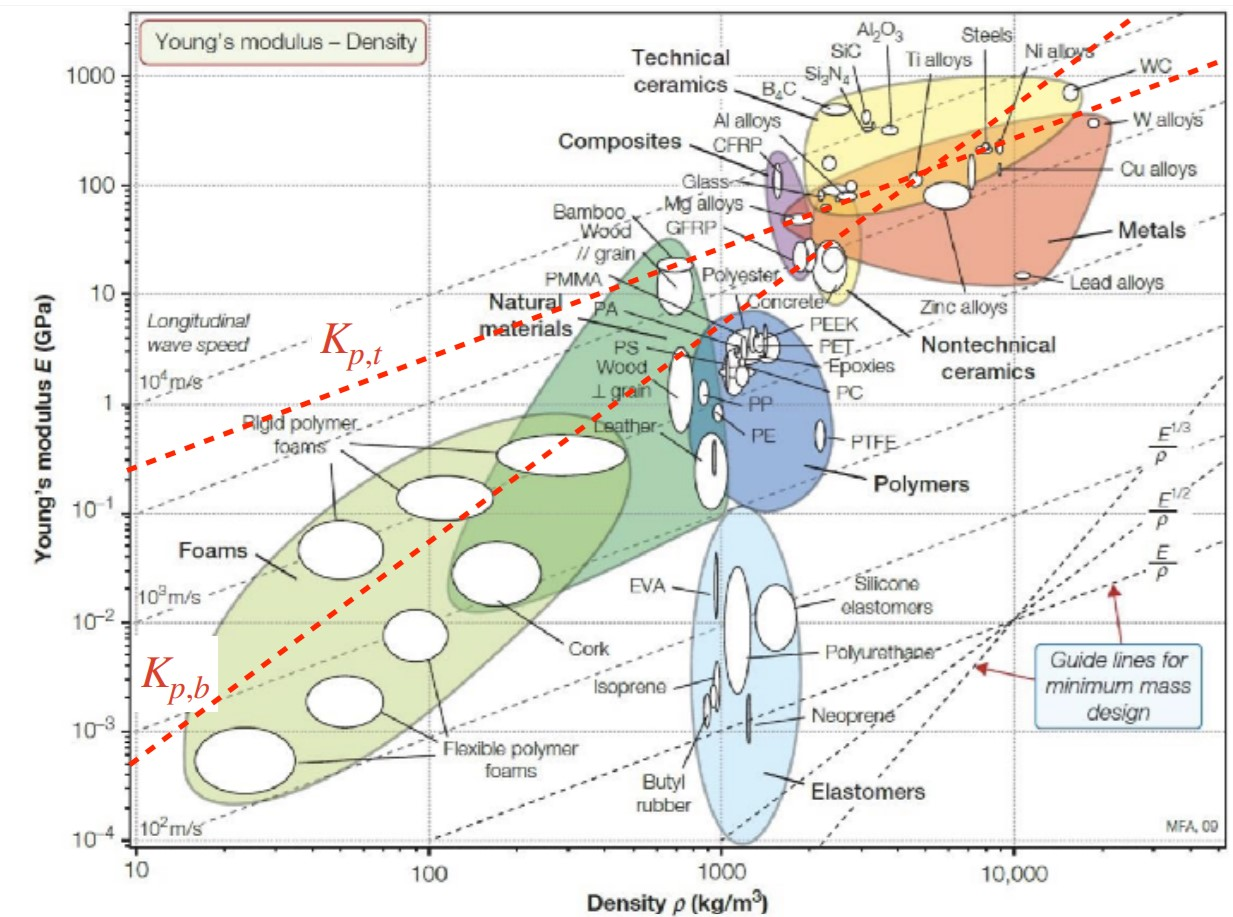
\includegraphics[width=11cm]{ashby}
		\caption{example of an Ashby map relating the density $\rho$ with the Young's module $E$ of different materials.} \label{fig:dist:ashby}
	\end{figure}
	
	\paragraph{Ashby performance index} In general, as example, a bar responds differently depending on the kind of load applied; considering a bar subjected to a pure tension load $P$, the stress state $\sigma$ and the weight $w$ can be evaluated as
	\[ \sigma = \frac P A \qquad \qquad w = \rho A L  \qquad \qquad \Rightarrow \quad w = \rho \frac P \sigma L = LP \frac \rho\sigma = \frac{LP}{K_{p,t}} \]
	In this relation the term $K_{p,t} = \sigma/\rho$ is the coefficient that relates material stiffness response (in a pure tension scenario) and it's mass $w$. Similarly if the bar is subjected to a pure bending moment $M$ we can define	
	\[ \sigma = -\frac {M}{I}y \qquad \qquad w = \rho A L  \qquad \qquad \Rightarrow \quad w = \sqrt{6MbL^2} \frac{\rho}{\sqrt{\sigma}} =  \frac{ \sqrt{6MbL^2}}{K_{p,b}}  \]
	In this case the coefficient $K_{p,b} = \sqrt \sigma/\rho$ refers to the coefficient that relates the material with equal mass to their stiffness response over the same bending moment. In figure \ref{fig:dist:ashby} is possible how the coefficient $K_{p,t}$ and $K_{p,b}$ can be used to determine materials that will result in same stiffness/mass behaviour.
	
	\paragraph{Chetwynd histograms} This kind of histograms (figure \ref{fig:dist:Chetwiynd}) reports different properties for two different materials: a bar going downward means that the first material is worst than the second (while if it's upward the response is better).
	
	\begin{SCfigure}[2][bht]
		\centering 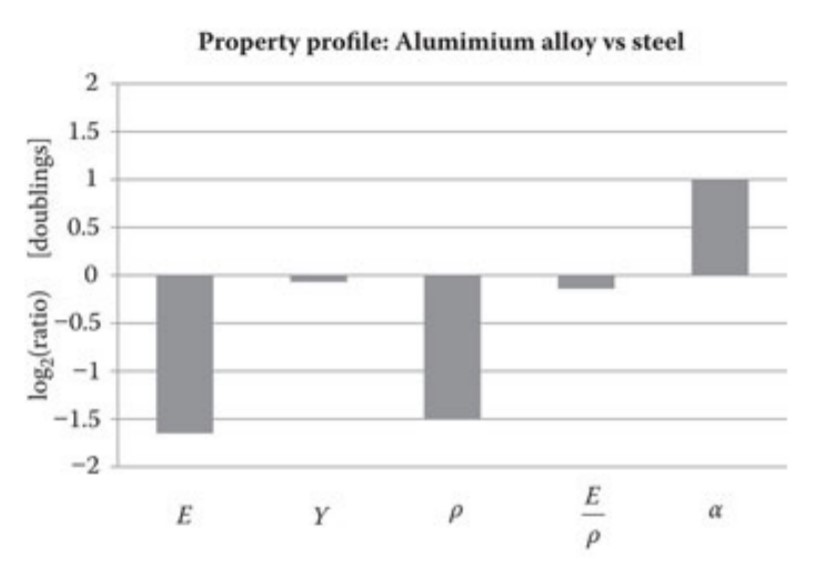
\includegraphics[width=6cm]{Chetwiynd}
		\caption{example of Chetwiynd histogram that compares aluminium alloys versus the steels one.} \label{fig:dist:Chetwiynd}	
	\end{SCfigure}
	
	In general vertical axis is logarithmic in order to focus on significant differences between materials. Properties, or \textbf{property groups}, are identified on the basis of selected use cases, factoring out any geometrical detail from the model.The underlying assumption is that, thanks to superposition of effects principle, the amount of change in behaviour by changing the material is not affected by the shape complexity.
	
	As example the tensile strength $\delta = \frac{Fl}{EA}$ of a bar relates only to the Young's module $E$ as property of the material,  and so can be evaluated in that property group. Another example is the maximum bending moment $M_{max}= \frac{2YI}{d}$ that's behave in the property group of the yielding strength $Y$. Also rational group properties can be defined like $\sqrt{E/\rho}$ that relates to the natural frequency of a beam. In general the typically considered property groups are
	\[ E \quad Y \quad \frac E \rho \quad \frac{\sqrt E}{\rho} \quad \frac{\sqrt[3] E}{\rho} \quad \frac Y E \quad \frac Y\rho \quad \frac k {cp} \quad \frac{cp}{\alpha} \quad \frac k\alpha \quad \frac k{\alpha E} \quad \frac 1 \alpha \quad \frac{1}{\alpha E} \]
	
	In general a way to pick the \textit{best} material for a specific application is to create a good-nut-not-excellent model material (that doesn't necessarily exists in real life) and confront him with a variety of real materials in order to find the one that suits most the application. As example figure \ref{fig:dist:chetcompr} compares a model material described in table \ref{tab:dist:modelmaterial} to spring steel.
	
	\begin{SCfigure}[2][bht]
		\centering 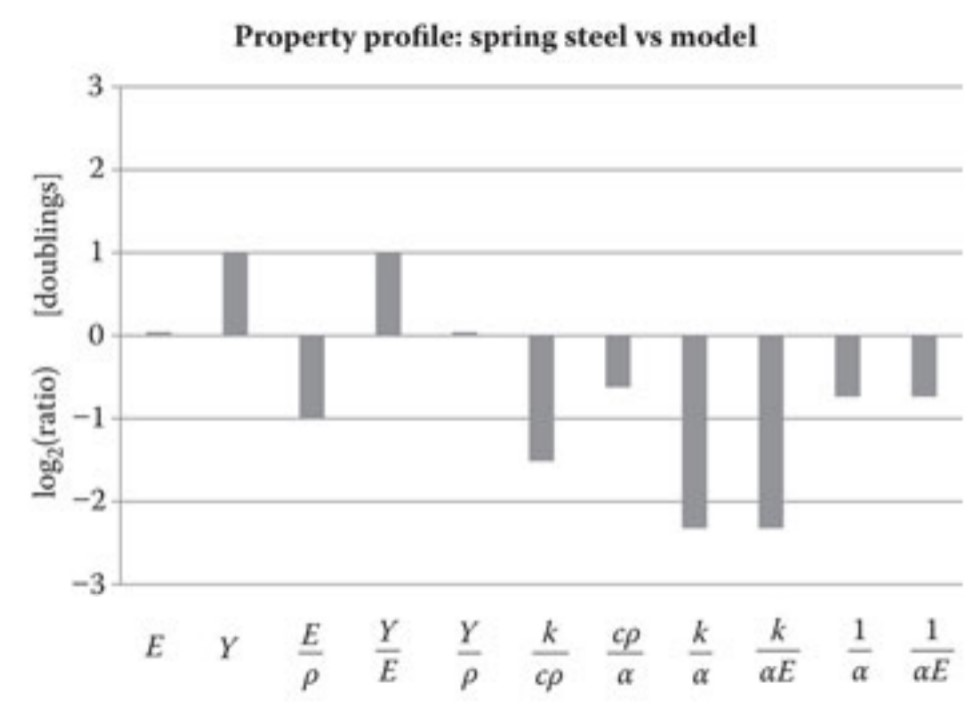
\includegraphics[width=6cm]{chet-model}
		\caption{example of Chetwynd histogram comparing spring steel and model material (table \ref{tab:dist:modelmaterial}).} \label{fig:dist:chetcompr}
	\end{SCfigure}
	
	\begin{table}[bht]
		\centering
		\caption{properties of the model material.} \label{tab:dist:modelmaterial}
		
		\begin{tabular}{r c | c | c }
			\textbf{Property} && \textbf{Typical of} & \textbf{Model value} \\ \hline
			modulus of elasticity & $E$ & mild steel & $200 GPa$ \\
			yield strength & $Y$ & mild steel & $300 MPa$ \\
			density & $\rho$ & oxide ceramic & $400 kg/m^3$ \\
			thermal expansion & $\alpha$ & oxide ceramic & $7\cdot 10^{-6} K^{-1}$ \\
			thermal conductivity & $k$ & Aluminum alloy & $150 W / m \, K$ \\
			specific heat & $c$ & many metals & $750 J / kg\, K$ \\
		\end{tabular}
		
	\end{table}
	
	
	\paragraph{Relevant metallic materials} For precise application the main materials are 
	\begin{itemize}
		\item steel: rather common due to availability, cost, ease of manufacture; it's an average performer;
		
		\item stainless steel: corrosion resistants and the non-magnetic property; usually the have worse performances and thermal property groups (compared to steel).
		
		\item cast iron: suitable for casting larger parts (such machine bases); it's pro's are the stability in time, the absorption of energy due to the graphite and the high damping coefficients;
		
		\item aluminum alloys: 2/3 times more costly than mild steel, similar to stainless steel, but lighter and with good thermal property groups (and so it's suitable for metrology loops  with lightly loaded structural loops);
		
		\item bronze and brass: were common precision materials due to their machinability and stability, while now are less common due to the technology improvement;
		
		\item tungsten: usually used as a thin film as buffer layer for accommodating thermal stresses;
		
		\item molybdenum: balanced perform respect to all metals;
		
		\item gold, platinum: thin layers or coatings to provide a particular surface layer functionality (such electrical, optical, electro-chemical, biocompatible ones);
		
		\item titanium alloys: marginally better than aluminum in mechanical property groups but word performer in thermal properties;
		
		\item INVAR (Iron, $36\%$ nickel alloy): similar to inox steels but with lower thermal expansion coefficient ($10$ times smaller).
	\end{itemize}
	
	Polymers and composites can also be used due to their low costs and the ability of produce complex shapes. \textbf{AGGIUNGERE}
	
	
	
	
	
	
	
	
	
	
	
	
	
	


\section{Isolation}
	
	The performance of a precision machine depends on the \textbf{attenuation} of the \textbf{environmental disturbances} acting upon it; this attenuation is performed by \textbf{isolators} (like the simple example in figure \ref{fig:dist:isolator}) which have to be designed according to the system dynamics.
	
	\begin{SCfigure}[2][bht]
		\centering
		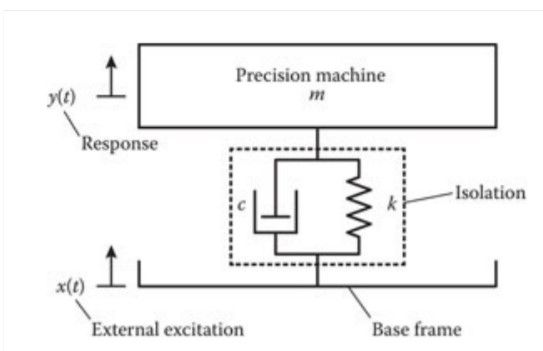
\includegraphics[width=5.5cm]{isolator}
		\caption{simple schematic of an isolator element connecting a precision machine to a base frame.} \label{fig:dist:isolator}
	\end{SCfigure}
	
	Considering the system in figure \ref{fig:dist:isolator}, its dynamic equation is $m\ddot y + c\dot y + ky = c\dot x + kx$ that, using the Laplace transform, determines the following transmissibility \de{transfer function}
	\begin{equation}
		H(s) = \frac{\text{output}}{\text{input}} =\frac{Y(s)}{X(s)} = \frac{cs + k}{ms^2 + cs +k}
	\end{equation}
	Substituting $s$ with the complex frequency $j\omega$ it's possible to define the \textbf{natural frequency} $f_0$ of the system and it's \textbf{damping ratio} $\zeta$ as
	\begin{equation}
		f_0 = \frac{\omega_0}{2\pi} =  \frac 1 {2\pi}\sqrt{\frac k m}  \qquad \qquad \qquad \zeta= \frac{c}{2\sqrt{km}}
	\end{equation}
	With this valued computed we can use Bode's diagram to represent the complex transfer function with his magnitude and phase (as in figure \ref{fig:dist:isolbode})
	
	\begin{SCfigure}[2][bht]
		\centering 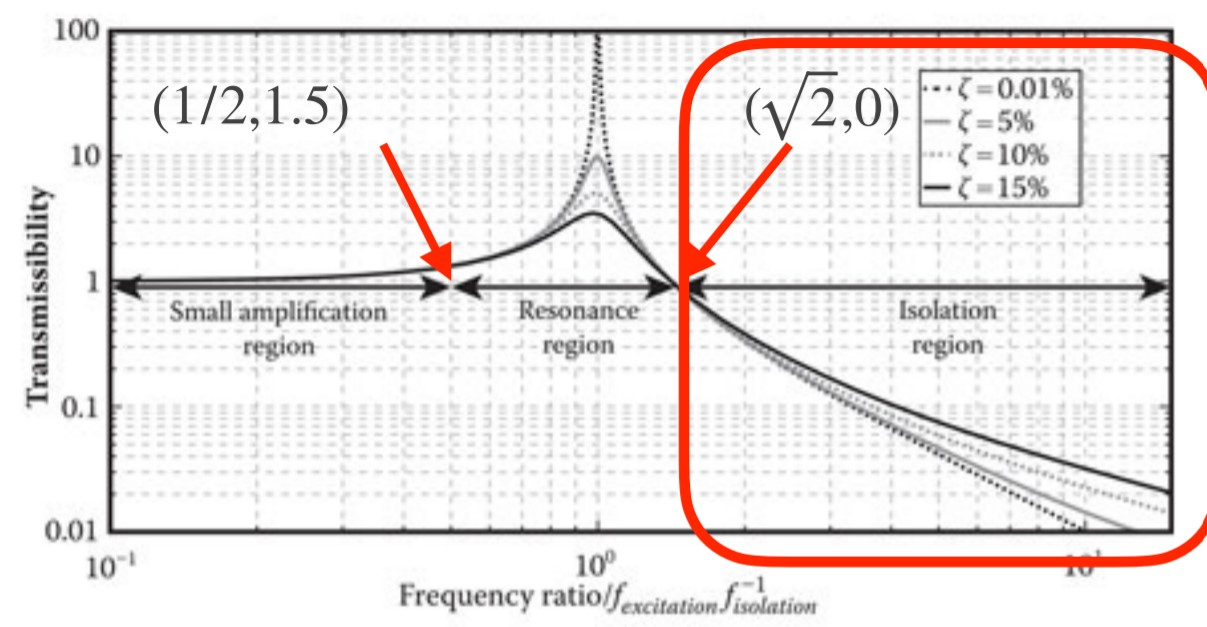
\includegraphics[width=7cm]{isol-response}
		\caption{transmissibility of a simple isolator depending on the damping ration $\zeta$.} \label{fig:dist:isolbode}
	\end{SCfigure}
	
	As we can see at the natural frequency $f_0$ there's the \de{resonance} phenomena that, given a fixed input, determines a very high output. The transmissibility function $T_d$ can be rewritten as
	
	\textbf{AGGIUNGERE LE EQUAZIONI}
	
	
	\paragraph{Isolating table} An \de{isolating table} (or bench) is an implementation, typically self-levelling, that uses a relatively large mass grounded through a damped spring. Usually precision equipment is placed on top of this kind of benches.
		
	\textbf{AAGGIUNGERE GIGURA}
	
	If we consider that on top of this table are put not infinitely stiff precision system, than the transmissibility function becomes more complex
	
	
	
	
	
	
	
	
	
	
	
	
	
	
	
	
	
	
	
	\part{Digital Manufacturing}
	\chapter{Industry 4.0}
	\de{Digital manufacturing} is the evolution of manufacturing where an \textbf{integrated approach} is centered around a computer system. The evolution can be seen from purely mechanical machinery, to \textbf{CNC} \textit{computer numerical controlled} machines up to system of computer-controlled machines.	
	
	Digital manufacture goes in the framework of \de{Industry 4.0}, the fourth industrial revolution that politically \textit{started} in 2013 after Angela Merkel's request in 2011 at the \textit{Hannover Messe}. The final report of the \textit{Industrie 4.0} committee defines
	\begin{itemize}
		\item design principles;
		\item challenges;
		\item impacts
	\end{itemize}
	that industry 4.0 present.
	
	\paragraph{Objectives} The main goals of this fourth industrial revolution can be summarized as
	\begin{itemize}
		\item the political idea of re-shoring of added value in western countries after the 2008 economical crises and in order to re-establish independence from chines production;
		\item sustain the salaries of both workers and the middle-class;
		\item sustain the e-commerce;
		\item mass customization; this has been possible after a change of mentality in production: previously products were massively fabricated, stocked and only finally sold for a \textit{high} amount of time while now the time delay between production and final customer is reduced, improving the customization of the products;
		\item related to the previous point, a goal is to compress the life cycle of the product in order to make it available faster to the customers.
		
	\end{itemize}
	
	\paragraph{Design principles} The main design principle driving the industry 4.0 are:
	\begin{itemize}
		\item the \textbf{interoperability} exemplified by the \textit{Internet of Things} \de{IoT}, the \textit{Industrial IoT} \de{IIoT} and the \textit{Internet of People} \de{IoP}; this principle has the goal to increase the efficiency in communication between machines (\textit{things}) or persons (\textit{people}) with the goal to reduce the number of operators needed in a plant;
		\item the implementation of \textit{Cyber-Physical Systems} \de{CPS}, mechatronic machines allowed to communicate and exchange information in order to improve the production chain;
		\item the information transparency using \textbf{public} and \textbf{open protocols} that allows CPS to communicate with each-other using an unified \textit{language}. The realization of \textbf{digital twins} as a model that simulate the behaviour of a real cyber-physical system is also important in order to estimate how the whole components will interact together;
		\item the implementation of \textbf{self-support} and \textbf{in-line help} to guide the operators in troubleshooting errors that might occur during normal functioning;
		\item the \textbf{decision de-centralization} giving autonomy to CPS in order to make machines perform trivial choices according to a specific stratification and prioritization of the tasks, allowing humans to better focus on problems that need an high supervision.
	\end{itemize}
	
	This design principle can somehow related to \textit{the Yardstick of Automation}, an article published in 1962 by \textit{Amber\&Amber} that relates the order of automation by evaluating the human attributes that machines can substitute; such order are reported in table \ref{tab:ind:amber}. At this stage, with the industry 4.0, we consider industries between order 4 to 6 of that table.
	
	\begin{table}[bt]
		\centering
		\tabrule
		\caption{order nd related human attribute substituted (with example) according to "the Yardstick of Automation" article.} \label{tab:ind:amber}\vspace{2mm}
		\begin{tabular} { c c p{10cm} }
			Order & Human Attribute &  Example \\ \hline
			0 & none & manual tools \\
			1 & energy & powered machines and tools \\
			2 & dexterity & single-cycle automatics (\textit{dexterity} means \textit{self-feeding} in a sense of repeatable system) \\
			3 & diligence & repeats cycle, open-loop control; ability to perform all the action with the same accuracy \\
			4 & judgment & closed loop, numerical controls, self-measuring systems \\
			5 & evaluation & computer control, model of process required for automation \\
			6 & learning & limited self-programming and some artificial intelligence \\
			7 & reasoning & inductive reasoning (cause $\rightarrow$ effects) \\
			8 & creativity & performing original designs unaided \\
			9 & dominance & machine is a master
			
		\end{tabular}	
		
		\vspace{2mm}
		\tabrule
	\end{table}
	
	\paragraph{Challenges} At this stage the main challenges of industry 4.0 are:
	\begin{itemize}
		\item cybersecurity: cyber-physical systems are \textit{high-tech} equipment that has the weakness of being hacked with so the possibility of high damages to production and operators;
		\item reliability and resiliency of the communication \textit{machine-to-machine} \textbf{M2M} mainly determined by the bandwidth of communication but most importantly it's latency;
		\item system should be design with a drop-in, plug-in approach on existing processes; plants cannot be re-invented from scratch in order to introduce a new machine, but all the pieces should be able to work together following the same unified protocols and standards;
		\item the protection of the intellectual property (that's put in danger with the high frequency of exchanging digital files);
		\item the reluctancy of plant owner to change the way industry processes are made and the need of re-train operators;
		\item the initial loss of labor that will be in the years reconverted into a \textit{higher order} operators.
	\end{itemize}
	
	\paragraph{Impacts} The main impacts provided by industry 4.0 can be summarized in:
	\begin{itemize}
		\item \textit{servitization} as the passage from selling goods to selling services to people;
		\item the productivity and its resilience;
		\item safety for human operators;
		\item integrated design of product and process (the two things now will go together and shouldn't be consider as separate);
		\item the cos structure in terms of money allocation in the production process;
		\item the socio-economical factors;
		\item the ability to have a high number of data to analyse and process.
	\end{itemize}
	
\section*{Digital manufacturing and industry 4.0} 
	Regarding industry 4.0 and digital manufacturing some core enable technology are common such the M2M connectivity between cyber-physical system, the connectivity layer provided by the industry internet of things, the additive manufacturing as the dematerialization of the design and the machine learning/artificial intelligence to make autonomous decision possible.
	
	\paragraph{CPSs} Cyber-physical systems are mechatronic system, so mechanisms whose actuators are controlled by a computer system based on output from sensors and logics provided by algorithms. Digital manufacturing enables CPSs must be IoT-connected in order to provide the plant controller with information its own status and accept incoming tasks. \\
	The industrial internet of things has to support communication (M2M) between a number of CPSs that can be theoretically huge. In this sense \de{IP protocols} standard have been created allowing $4.3\cdot 10^9$ addresses for \texttt{IPv4} version and more recently \texttt{IPv6} allowing $3.4\cdot 10^{38}$ unique addresses.
	
	\subsection*{Networking model}
		According to the internet model, data can be exchanged between machines by creating a networking stack where the package is composed by 4 different layers stacked (as shown in figure \ref{fig:ind:netstack}).
		\begin{SCfigure}[2][b]
			\centering 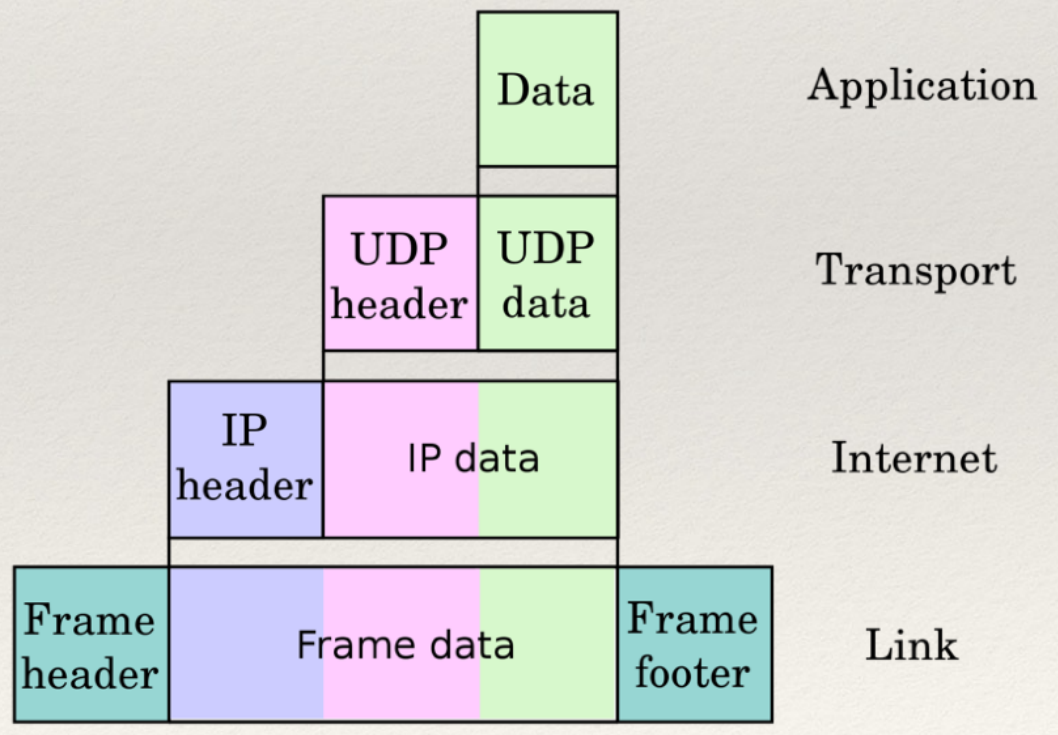
\includegraphics[width=6cm]{net-stack}
			\caption{4 layers and related package constitution used for communication using internet protocols.} \label{fig:ind:netstack}
		\end{SCfigure}
		Such layers are:
		\begin{itemize}
			\item[\texttt{L1})] link layer made by the physical carrier standard (such Ethernet cable or WiFi) and it's protocol (\texttt{MAC}, \texttt{813.11}, \texttt{ARP}...) that explains \textit{how} data are transmitted;
			\item[\texttt{L2})] internet (network) layer made by the addressing protocols (such \texttt{IPv4}, \texttt{IPv6} or \texttt{ICMP}) in order to properly address packages of information;
			\item[\texttt{L3})] transport layer (\texttt{TCP}, \texttt{UDP} protocols) that manages the connection between nodes in the network;
			\item[\texttt{L4})] application layer (such \texttt{HTTP}, \texttt{FTP}, \texttt{IMAP}, \texttt{LDAP} standards) that describes and contains encoded data.
		\end{itemize}
	
		The industrial internet of things must support communications between cyber-physical systems with a M2M communication; for the first layer \texttt{L1}, the link should be \textit{as fast as possible} in order to have a low latency and for this reason the new 5G protocol seems promising. Regarding instead the application layer \texttt{L4} protocols we can use the  more verbose and complex standard such \texttt{REST} or more lightweight ones (such \texttt{MQTT}, \texttt{ZeroMQ}, \texttt{AMQP} and \texttt{OPC-UA}).
	
		\paragraph{REST and HTTP overhead} The REST (\textit{REpresentational State Transfer}) is a protocol extended from HTTP and is characterized by a verbose (large) overhead, a complex syntax and by a connection $n$ machine to 1 server. The communication starts by sending 3 first packages for a hand-shake communication synchronization (no information are exchanged at this point) and only after this operation data are exchanged between one machine and the server. The headers of this communication is large: considering in fact that the simplest request phrase requires 14 bytes, the associated full request stack is made by 437 bytes (need of bigger bandwidth) and the number of packages sent back-and-forth between machine and server is \textit{high}, resulting in higher latency.
		
		The combination of handshaking protocols and verbose frame headers/footers allows to have a reliable and robust connection with a needed increase of bandwidth and with an increased latency; for this reason more \textit{machined based} protocols have been implemented in order to reduce latency while exchanging information between server and machines with the draw-back of reducing the number of packages sent resulting in less synchronization and confirmation (for example of package delivered).
	
		In IoP messages are frequently \textit{heavy} and seldom and the robustness of the HTTP protocol allows to better adapt the information exchanged between machines using different web servers or browsers. On the other hand IoT requires smaller messages sent with high frequency and so standard are enforced to minimize possible sources of unexpected conditions while still maintaining low latency.
		
		In IIoT messages also should follow routes more complex than $n$-to-1 ($n$ clients to 1 server) and so we need to minimize the overhead and support flexible topologies of the network infrastructure. A way to perform this operation is by using \textbf{message queuing protocols} (such \texttt{MQTT}, \texttt{ZeroMQ}) where clients can be both \textbf{publishers} and/or \textbf{subscribers} of the information; all this communication system is handled by the so called \textbf{broker}.\\
		The idea behind such type of communication is that clients that join a broker as publisher can send information to this intermediate server that immediately notifies all the subscribed machined with the information provided.
	
	
	
	
	
	
	
	
	
	
	
	
	
	
	
	
	\chapter{Manufacturing Systems}
	
	To give a shape shape to a block of raw material, namely \textit{\textbf{workpiece}}, various methods can be used involving a different required number of \de{motion axis}:
	\begin{itemize}
		\item the \textbf{forming} processes that are based on the plastic deformation of the workpiece requires at least 1 motion axis. In this course such manufacturing process is skipped because the motion planning and control is (usually) trivial;
		\item \textbf{subtractive} processes are based on the removal of material from the workpiece and usually requires 2.5 motion axis or more;
		\item we can add more material to the existing block using \textbf{additive manufacturing} techniques that, as for subtractive processes, requires at least 2.5 motion axis.
	\end{itemize}
	In subtractive/additive manufacturing there is a \de{tool} performing the process (such mills, polarized wires, extruding nozzles...) whose motion is performed by a synchronized action of two or more axes (typically in cartesian arrangement); the union of \textbf{trajectory} and \textbf{speed} of the tool represent it's \de{motion} that must be planned according to \textbf{geometry} and \textbf{process specifics}.
	
	
\section{Machining}
	
	The majority of products involves the \de{machining} process either directly or indirectly; machining involves a combination of linear and rotary motion and can be split in 3 main operational categories:
	\begin{itemize}
		\item \textbf{turning} where the workpiece is rotating and the tool is displacing; a good example of turning machining is the lathe (\textit{tornio});
		\item in \textbf{drilling} and \textbf{milling} the tool is rotating and there is a combined relative displacement between tool and workpiece.
	\end{itemize}
	The mechanism of \textbf{chip formation} (\textit{formazione di trucioli}) generated by this processes depends on multiple \textbf{tool parameters} such:
	\begin{itemize}
		\item the relative speed of the tool and the workpiece, namely the \textbf{cutting speed};
		\item the cross section of the removed material
	\end{itemize}
	This tool parameters strictly depends on the \textbf{machining parameters} as trajectory, rotation and translation speeds.
	
	\subsection*{Turning}
		
		While dealing with \textbf{turning}, considering the scheme in figure \ref{fig:man:turning}, the main machining parameters are the spindle speed, the feed rate and the spindle power.
		
		\begin{SCfigure}[2][bht]
			\centering 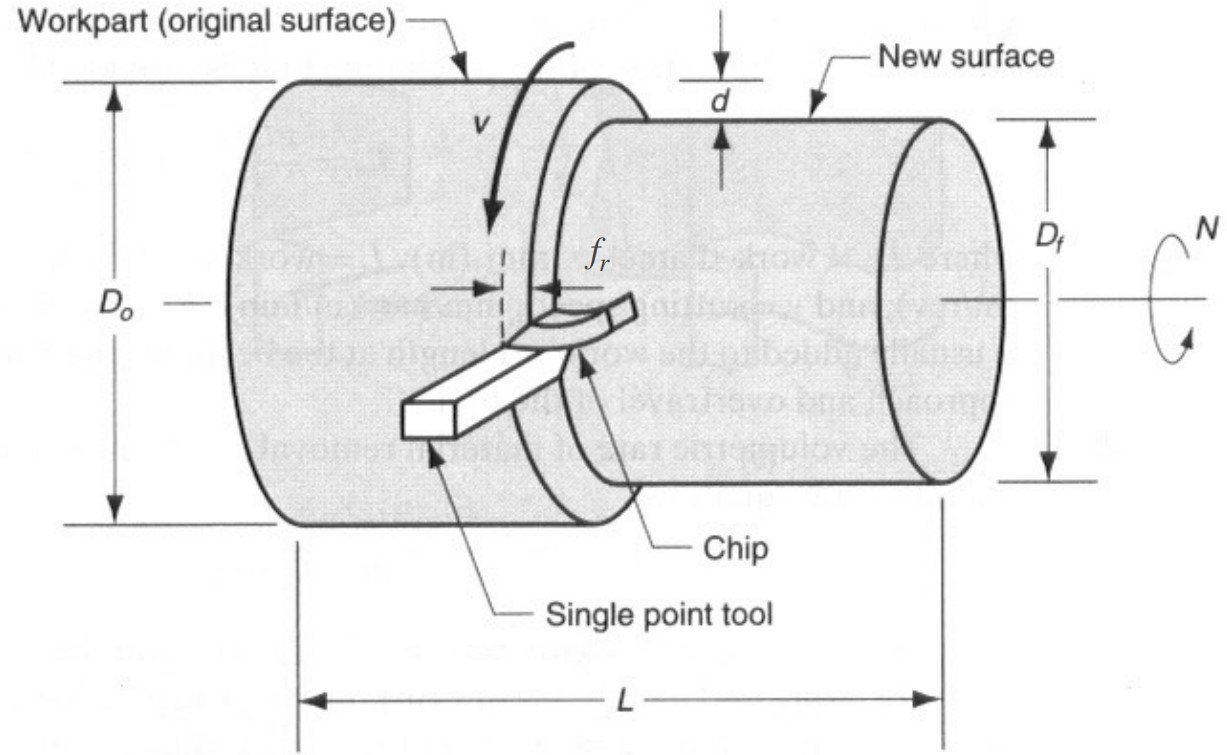
\includegraphics[width=7cm]{turning}
			\caption{main dimensions and parameters used for the calculation on turning's machining parameters.} \label{fig:man:turning}
		\end{SCfigure}
	
		
		
		\begin{table}[bht]
			\centering
			\tabrule
			\caption{formulas for machining systems} \vspace{2mm}
			\begin{tabular} {M{3cm} M{3cm} M{3cm} M{3cm}}
				Parameter  & Turning & Milling & Drilling \\ \hline
				$v(m/min)$ & $\pi D_0 N$ & $\pi D N$ & $\pi D N$ \\
				$N(1/min)$ & $\frac{v}{\pi D_0}$ & $\pi D N$ & $\pi D N$ \\
				
			\end{tabular}	
				
			\vspace{2mm}
			\tabrule
		\end{table}
	
	
	
	
	
	
	
	
	
	
\end{document}